% ============================================================================
% paper.tex
% Robustness of VLM Encoders to Combined Image Corruptions
%
% КОМПИЛЯЦИЯ (обязательно именно так, иначе ссылки не появятся!):
%   pdflatex paper
%   bibtex paper
%   pdflatex paper
%   pdflatex paper
% ============================================================================
\documentclass[10pt, twocolumn]{article}

% ---- Encoding ----
\usepackage[utf8]{inputenc}
\usepackage[T1]{fontenc}
\usepackage{times}

% ---- Page layout ----
\usepackage[
  top=1in, bottom=1in,
  left=0.75in, right=0.75in
]{geometry}

% ---- Math ----
\usepackage{amsmath, amssymb, amsthm}

% ---- Graphics ----
\usepackage{graphicx}
\usepackage{subcaption}
\usepackage{float}
\graphicspath{{results_combined_corruptions/}}  % папка с графиками

% ---- Tables ----
\usepackage{booktabs}
\usepackage{multirow}
\usepackage{array}

% ---- Typography ----
\usepackage{microtype}
\usepackage{xcolor}
\usepackage{enumitem}
\usepackage{balance}

% ---- Captions ----
% Таблицы: подпись СВЕРХУ
% Рисунки: подпись СНИЗУ
\usepackage{caption}
\captionsetup[table]{position=top,  labelfont=bf, font=small, skip=4pt}
\captionsetup[figure]{position=bottom, labelfont=bf, font=small, skip=4pt}

% ---- Hyperlinks (ПОСЛЕДНИМ из пакетов!) ----
\usepackage{hyperref}
\usepackage{cleveref}
\hypersetup{
  colorlinks = true,
  linkcolor  = blue!60!black,
  citecolor  = blue!60!black,
  urlcolor   = blue!60!black
}

% ---- BibTeX: IEEE нумерованный стиль [1] ----
% ВАЖНО: \bibliographystyle должен быть ДО \bibliography
% и оба должны быть в конце документа

% ---- Useful macros ----
\newcommand{\ie}{\textit{i.e.}}
\newcommand{\eg}{\textit{e.g.}}
\newcommand{\etal}{\textit{et al.}}
\newcommand{\cI}{\mathcal{I}}          % interaction effect symbol

% Colorblind-safe highlight (Okabe-Ito)
\definecolor{supercolor}{RGB}{213,94,0}   % оранжево-красный
\definecolor{subcolor}{RGB}{0,114,178}    % синий

% ============================================================================
\begin{document}

% ============================================================================
% TITLE
% ============================================================================
\title{
  \textbf{When Corruptions Compound: Superadditive Degradation of\\
  Vision-Language Encoders under Combined Image Corruptions}
}

\author{
  Kudinov Ruslan\\
  \textit{Innopolis University}
}
\date{}
\maketitle

% ============================================================================
% ABSTRACT
% ============================================================================
\begin{abstract}
Existing robustness benchmarks for Vision-Language Models~(VLMs),
including ImageNet-C~\cite{hendrycks2019benchmarking} and
RobustBench~\cite{croce2021robustbench}, evaluate models under
\emph{individual} image corruptions applied in isolation.
Real-world deployments, however, routinely impose
\emph{multiple simultaneous} corruptions---sensor noise
co-occurring with fog, motion blur combined with low contrast.
We present the first systematic study of
\emph{pairwise corruption interactions} for CLIP-family encoders
under zero-shot classification.
Using three OpenCLIP~\cite{ilharco2021openclip} models
(ViT-B/32, ViT-B/16, ViT-L/14) and seven corruption types
at three severity levels, we evaluate all $\binom{7}{2}=21$
pairwise combinations and quantify \emph{interaction effects}
as the gap between observed and expected (additive) accuracy drops.
Our key findings are:
(i)~\textbf{Superadditivity is real}---at low severity,
up to 8~of~21 pairs degrade accuracy worse than the sum of
individual drops;
(ii)~\textbf{contrast\,+\,shot\_noise} is the most dangerous
pair across all architectures (interaction up to $+0.227$);
(iii)~\textbf{model scale amplifies superadditivity}---ViT-L/14
shows twice the interaction effect of ViT-B/32;
(iv)~\textbf{floor effects suppress superadditivity} at high
severity, revealing a regime transition absent from current
benchmarks;
(v)~\textbf{corruption order is critical}---4 of 5 top pairs
are order-sensitive, with accuracy gaps up to~$0.21$ between
application orders, exposing a worst-case evaluation gap in
existing protocols.These findings collectively expose systematic blind spots
absent from all existing VLM robustness benchmarks,
including ImageNet-C~\cite{hendrycks2019benchmarking},
CCC~\cite{press2023rdumb}, and related work on
augmentation--corruption interactions~\cite{chen2021augcorr}.
Code is available at
\url{https://github.com/anonymous/vlm-combined-corruptions}.
\end{abstract}

% ============================================================================
% 1. INTRODUCTION
% ============================================================================
\section{Introduction}
\label{sec:intro}

Vision-Language Models~(VLMs) such as CLIP~\cite{radford2021clip}
have demonstrated strong zero-shot generalization across visual
recognition benchmarks.
Their robustness to distribution shift has been studied through
ImageNet-C~\cite{hendrycks2019benchmarking}, which applies
15~corruption types at 5~severity levels, and
RobustBench~\cite{croce2021robustbench}, which tracks
state-of-the-art robustness over time.

\paragraph{The gap.}
A fundamental assumption of all existing corruption benchmarks is
that corruptions are applied \emph{one at a time}.
This assumption is violated in virtually every real-world
deployment scenario.
A camera on an autonomous vehicle simultaneously experiences
sensor noise, motion blur, and reduced contrast from adverse
weather.
A surveillance system processes frames degraded by JPEG
compression \emph{and} brightness variation.
\cref{fig:examples} illustrates these compound effects.

\paragraph{Research questions.}
\begin{enumerate}[leftmargin=*, label=\textbf{RQ\arabic*.}]
  \item Do pairwise corruption combinations degrade VLM accuracy
        \emph{superadditively}---worse than the sum of individual
        drops?
  \item Does model scale (ViT-B/32 $\to$ ViT-B/16 $\to$
        ViT-L/14) confer robustness against combined corruptions?
  \item Which pairs are most dangerous, and is the ranking
        consistent across architectures?
  \item Does the \emph{order} of corruption application affect
        outcomes?
\end{enumerate}

\paragraph{Contributions.}
\begin{itemize}[leftmargin=*]
  \item We introduce the \textbf{interaction effect} metric $\cI$
        for quantifying superadditivity in corruption pairs
        (\cref{sec:method}).
  \item We conduct the \textbf{first systematic pairwise
        evaluation} of combined corruptions for CLIP-family
        encoders in zero-shot classification.
  \item We identify \textbf{contrast\,+\,shot\_noise} as
        universally the most dangerous pair, with $\cI=+0.227$
        for ViT-L/14.
  \item We reveal a \textbf{severity-dependent regime
        transition}: superadditivity dominates at low severity
        and collapses at high severity.
  \item We demonstrate that \textbf{corruption order is
        critical}: 4 of 5 top pairs are order-sensitive,
        with worst-case accuracy gaps up to $0.21$.
  \item We show a \textbf{patch-size trade-off}: smaller
        patches improve noise robustness at the cost of
        JPEG robustness.
\end{itemize}

% ============================================================================
% 2. RELATED WORK
% ============================================================================
\section{Related Work}
\label{sec:related}

\paragraph{Corruption robustness benchmarks.}
Hendrycks and Dietterich~\cite{hendrycks2019benchmarking}
introduced ImageNet-C, applying 15~corruptions
\emph{independently} at 5~severity levels and aggregating
results via mean Corruption Error~(mCE).
This single-corruption protocol is inherited by
ImageNet-3DCC~\cite{kar2022imagenet3dcc},
RobustBench~\cite{croce2021robustbench}, and all subsequent
corruption benchmarks.

\paragraph{VLM robustness.}
Recent work has studied CLIP under distributional shift.
The ROZ benchmark~\cite{roz2024} evaluates zero-shot CLIP
under natural, synthetic, and adversarial shifts---all applied
individually.
BAT-CLIP~\cite{batclip2024} shows that zero-shot CLIP is
not robust to common corruptions under increasing severity,
again with independent corruptions.
A concurrent survey~\cite{wang2024survey} finds that
robustness does not necessarily scale with model size,
consistent with our results, but does not study combined
corruptions.

\paragraph{Combined corruptions.}
The Continuously Changing Corruptions (CCC)
dataset~\cite{press2023rdumb} combines pairs of corruptions
via random walks to benchmark \emph{continual test-time
adaptation}~(TTA) methods for CNNs.
CCC differs fundamentally from our work: it targets temporal
corruption streams for TTA evaluation on ResNet-50, and does
not quantify pairwise interaction effects.
\textbf{To the best of our knowledge, no prior work has
systematically quantified pairwise corruption interaction
effects for VLM encoders in zero-shot classification.}

% ============================================================================
% 3. METHODOLOGY
% ============================================================================
\section{Methodology}
\label{sec:method}

\subsection{Models}
We evaluate three OpenCLIP~\cite{ilharco2021openclip}
models trained on LAION-2B~\cite{schuhmann2022laion}:
\textbf{ViT-B/32} (patch size~32, 88M~params),
\textbf{ViT-B/16} (patch size~16, 86M~params),
and \textbf{ViT-L/14} (patch size~14, 307M~params).
All models use the prompt template
\texttt{"a photo of a \{class\}."} for zero-shot
classification.

\subsection{Dataset}
We use the CIFAR-100~\cite{krizhevsky2009learning}
test split (10{,}000 images, 100 classes), sampling
$N=1{,}000$ images with fixed seed~42.

\subsection{Corruption Protocol}
We use the \texttt{imagecorruptions}
library~\cite{michaelis2019dragon}, which implements the
ImageNet-C corruption suite.
Seven corruption types are selected:
\textit{noise} (\texttt{gaussian\-\_noise},
\texttt{shot\-\_noise}),
\textit{blur} (\texttt{motion\-\_blur}),
\textit{weather} (\texttt{fog}), and
\textit{digital} (\texttt{jpeg\-\_compression},
\texttt{brightness}, \texttt{contrast}).
Severity levels $s \in \{1,3,5\}$ are evaluated.

\textbf{Combined corruptions} apply two corruptions
sequentially:
\begin{equation}
  \mathbf{x}_{c_1 \to c_2}
  = \mathrm{corrupt}\!\bigl(
      \mathrm{corrupt}(\mathbf{x},\, c_1,\, s),\,
      c_2,\, s
    \bigr).
  \label{eq:combined}
\end{equation}
All $\binom{7}{2}=21$ pairwise combinations are evaluated.

\subsection{Interaction Effect Metric}
\label{sec:metric}

Let $\mathrm{acc}(\cdot)$ denote Top-1 accuracy.
The \textbf{accuracy drop} under corruption $c$ at severity
$s$ is:
\begin{equation}
  \Delta(c,s)
  = \mathrm{acc}_{\mathrm{clean}} - \mathrm{acc}(c,s).
  \label{eq:drop}
\end{equation}

Under the \textbf{additive independence assumption}, the
expected drop under combined corruptions would be:
\begin{equation}
  \Delta_{\mathrm{exp}}(c_1,c_2,s)
  = \Delta(c_1,s) + \Delta(c_2,s).
  \label{eq:expected}
\end{equation}

The \textbf{interaction effect} is:
\begin{equation}
  \cI(c_1,c_2,s)
  = \Delta(c_1{+}c_2,\,s)
    - \Delta_{\mathrm{exp}}(c_1,c_2,s).
  \label{eq:interaction}
\end{equation}

A pair is classified using threshold $\varepsilon = 0.005$:
\begin{align*}
  \cI >  +\varepsilon &\;\Rightarrow\;
    \textbf{superadditive} \\
  |\cI| \le \varepsilon &\;\Rightarrow\;
    \textbf{additive} \\
  \cI < -\varepsilon &\;\Rightarrow\;
    \textbf{subadditive}
\end{align*}

% ============================================================================
% 4. EXPERIMENTS & RESULTS
% ============================================================================
\section{Experiments \& Results}
\label{sec:experiments}

\subsection{Experimental Setup}
All experiments run on a single CUDA GPU with batch
size~64.
Text features are precomputed once per model.
Total compute: $\approx$111~minutes.

% -------------------------------------------------------
% TABLE 1 — Summary
% -------------------------------------------------------
\begin{table}[t]
\caption{
  Top-1 accuracy under clean, average single-corruption
  (7 types), and average combined-corruption (21 pairs)
  conditions at severity $s=1$.
  \textbf{Gap} = Single $-$ Combined.
}
\label{tab:summary}
\centering
\small
\setlength{\tabcolsep}{5pt}
\begin{tabular}{lcccc}
\toprule
\textbf{Model}
  & \textbf{Clean}
  & \textbf{Single}
  & \textbf{Combined}
  & \textbf{Gap} \\
\midrule
ViT-B/32 & 0.753 & 0.450 & 0.218 & 0.231 \\
ViT-B/16 & 0.788 & 0.473 & 0.239 & 0.234 \\
ViT-L/14 & \textbf{0.835} & \textbf{0.544} & \textbf{0.295} & \textbf{0.249} \\
\bottomrule
\end{tabular}
\end{table}

% -------------------------------------------------------
% TABLE 2 — Superadditivity counts
% -------------------------------------------------------
\begin{table}[t]
\caption{
  Number of superadditive / additive / subadditive pairs
  out of 21~total, per model and severity.
}
\label{tab:counts}
\centering
\small
\begin{tabular}{llccc}
\toprule
\textbf{Model} & \textbf{Sev.}
  & \textbf{Super}
  & \textbf{Add.}
  & \textbf{Sub} \\
\midrule
\multirow{3}{*}{ViT-B/32}
  & 1 & 8 & 3 & 10 \\
  & 3 & 0 & 0 & 21 \\
  & 5 & 0 & 0 & 21 \\
\midrule
\multirow{3}{*}{ViT-B/16}
  & 1 & 6 & 0 & 15 \\
  & 3 & 0 & 0 & 21 \\
  & 5 & 0 & 0 & 21 \\
\midrule
\multirow{3}{*}{ViT-L/14}
  & 1 & 7 & 2 & 12 \\
  & 3 & 1 & 0 & 20 \\
  & 5 & 0 & 0 & 21 \\
\bottomrule
\end{tabular}
\end{table}

% -------------------------------------------------------
% TABLE 3 — Top-5 superadditive pairs
% -------------------------------------------------------
\begin{table}[t]
\caption{
  Top-5 superadditive pairs by interaction effect $\cI$
  (\cref{eq:interaction}) at severity $s=1$.
  \textbf{Exp.}~= expected additive drop;
  \textbf{Real}~= observed drop.
}
\label{tab:top5}
\centering
\small
\setlength{\tabcolsep}{3pt}
\begin{tabular}{llccc}
\toprule
\textbf{Model} & \textbf{Pair}
  & \textbf{Exp.}
  & \textbf{Real}
  & $\cI$ \\
\midrule
ViT-L/14 & contrast+shot\_noise & 0.543 & 0.770
  & \textbf{+0.227} \\
ViT-B/16 & contrast+shot\_noise & 0.624 & 0.742 & +0.118 \\
ViT-B/32 & contrast+shot\_noise & 0.613 & 0.724 & +0.111 \\
ViT-L/14 & fog+shot\_noise      & 0.689 & 0.799 & +0.110 \\
ViT-B/32 & fog+contrast         & 0.330 & 0.419 & +0.089 \\
\bottomrule
\end{tabular}
\end{table}

% -------------------------------------------------------
% FIGURE 1 — Qualitative corruption examples
% -------------------------------------------------------
\begin{figure*}[t]
  \centering
  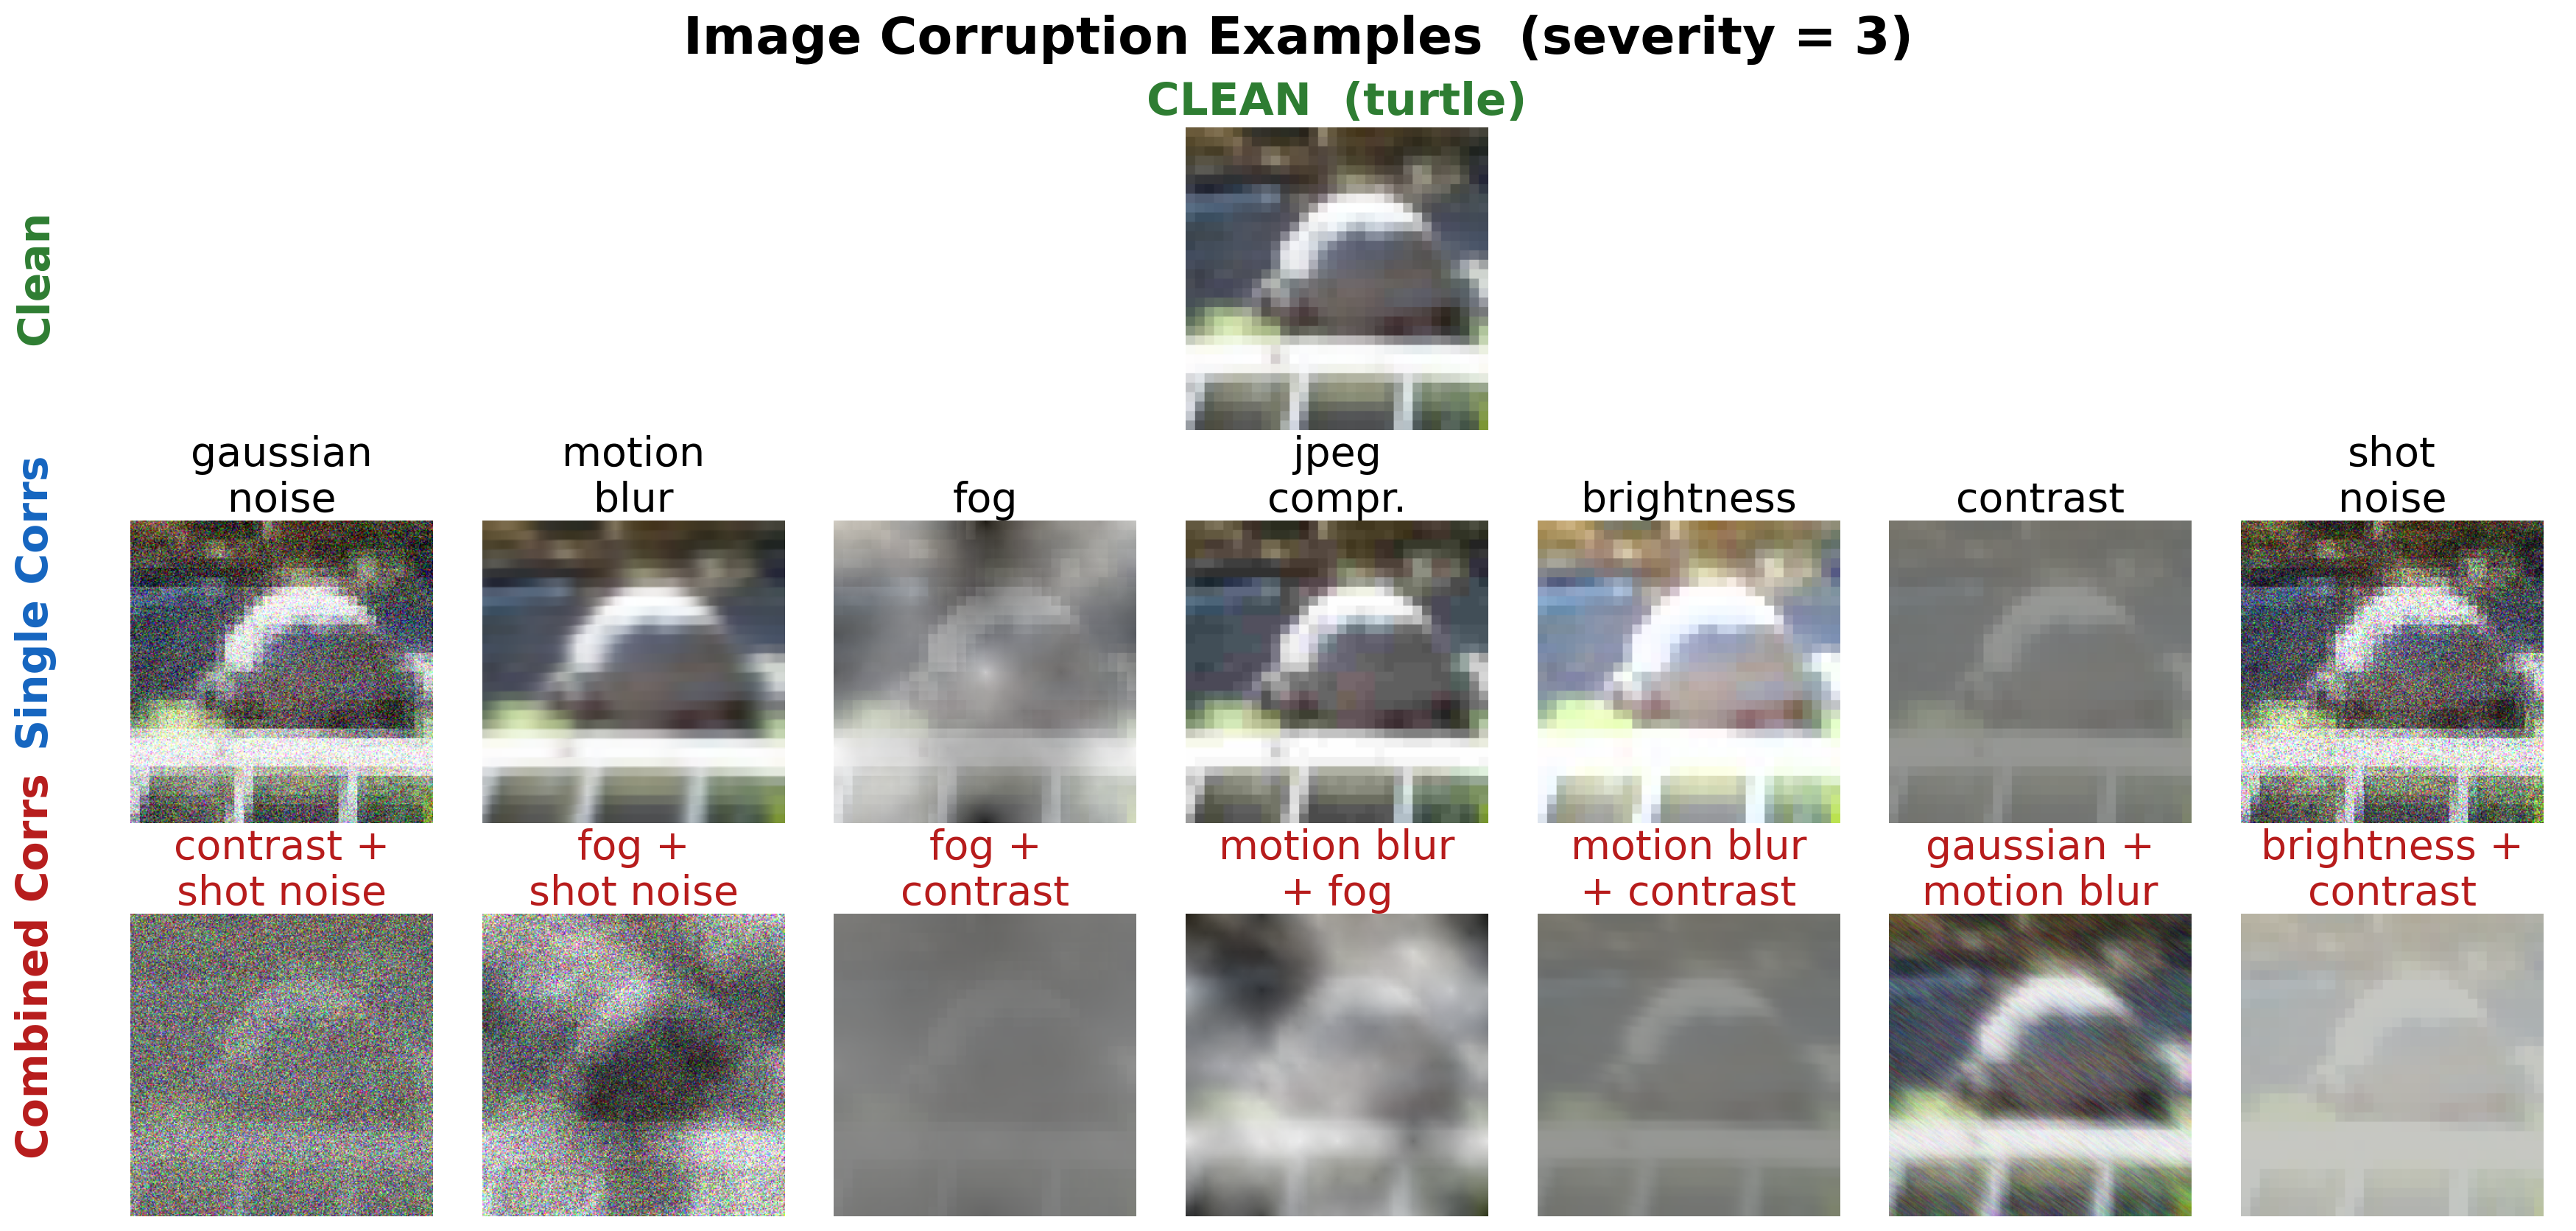
\includegraphics[width=\textwidth]{corruption_examples.png}
  \caption{
    Example images from CIFAR-100 under individual and
    combined corruptions at severity $s=3$.
    \textbf{Row 1}: clean.
    \textbf{Row 2}: single corruptions
    (left to right: gaussian\_noise, motion\_blur, fog,
    jpeg\_compression, brightness, contrast, shot\_noise).
    \textbf{Row 3}: selected pairwise combinations.
    Combined corruptions visually compound the degradation
    in ways not predictable from individual corruptions.
  }
  \label{fig:examples}
\end{figure*}

% -------------------------------------------------------
% RQ1 — Superadditivity
% -------------------------------------------------------
\subsection{RQ1: Is Superadditivity Real?}
\label{sec:rq1}

\cref{tab:counts} confirms that superadditivity is a
robust phenomenon at low severity ($s=1$): across all
three models, 6--8 of~21 pairs exhibit $\cI > 0.005$.
\cref{tab:top5} shows the five most dangerous pairs.

\textbf{contrast\,+\,shot\_noise} is the top-ranked
superadditive pair for \emph{all three} architectures,
with interaction effects of $+0.111$, $+0.118$, and
$+0.227$ for ViT-B/32, ViT-B/16, and ViT-L/14,
respectively.

At higher severity ($s \geq 3$), superadditivity
collapses to near-zero for all models
(\cref{tab:counts}).
We attribute this to a \textbf{floor effect}: at
high severity, individual corruptions already drive
accuracy near chance~($\approx 0.01$--$0.05$),
leaving no room for further combined degradation.
The full degradation picture is shown in
\cref{fig:heatmaps} (heatmaps) and
\cref{fig:severity} (severity curves).

% -------------------------------------------------------
% RQ2 — Scale
% -------------------------------------------------------
\subsection{RQ2: Does Scale Help?}
\label{sec:rq2}

\cref{tab:summary} shows that while ViT-L/14
achieves the highest clean accuracy
(+8.2~pp over ViT-B/32), the \textbf{Gap} between
single and combined corruptions is \emph{largest}
for the bigger model ($0.249$ vs.\ $0.231$).
ViT-L/14 also exhibits a substantially stronger
interaction for contrast\,+\,shot\_noise ($+0.227$)
than ViT-B/32 ($+0.111$).

\noindent\textbf{Finding 1:}
\textit{Scale does not protect against combined
corruptions.
Higher clean accuracy creates more headroom for
superadditive degradation, amplifying interaction
effects.}

% -------------------------------------------------------
% RQ3 — Most dangerous pairs
% -------------------------------------------------------
\subsection{RQ3: Which Pairs Are Most Dangerous?}
\label{sec:rq3}

The heatmaps in \cref{fig:heatmaps} reveal a
consistent ranking across architectures.
The most dangerous pairs invariably involve
\texttt{shot\_noise} combined with a moderate
structural corruption (\texttt{contrast},
\texttt{fog}).
Pairs of two already-severe corruptions
(\eg, \texttt{gaussian\_noise\,+\,shot\_noise})
tend to be \emph{subadditive} due to floor effects.
The interaction maps are further visualised in
\cref{fig:superadditivity}.
\cref{fig:crossmodel} directly compares interaction
effects across all three architectures, confirming
that ViT-L/14 consistently exhibits stronger
superadditivity than smaller models.

\begin{figure*}[t]
  \centering
  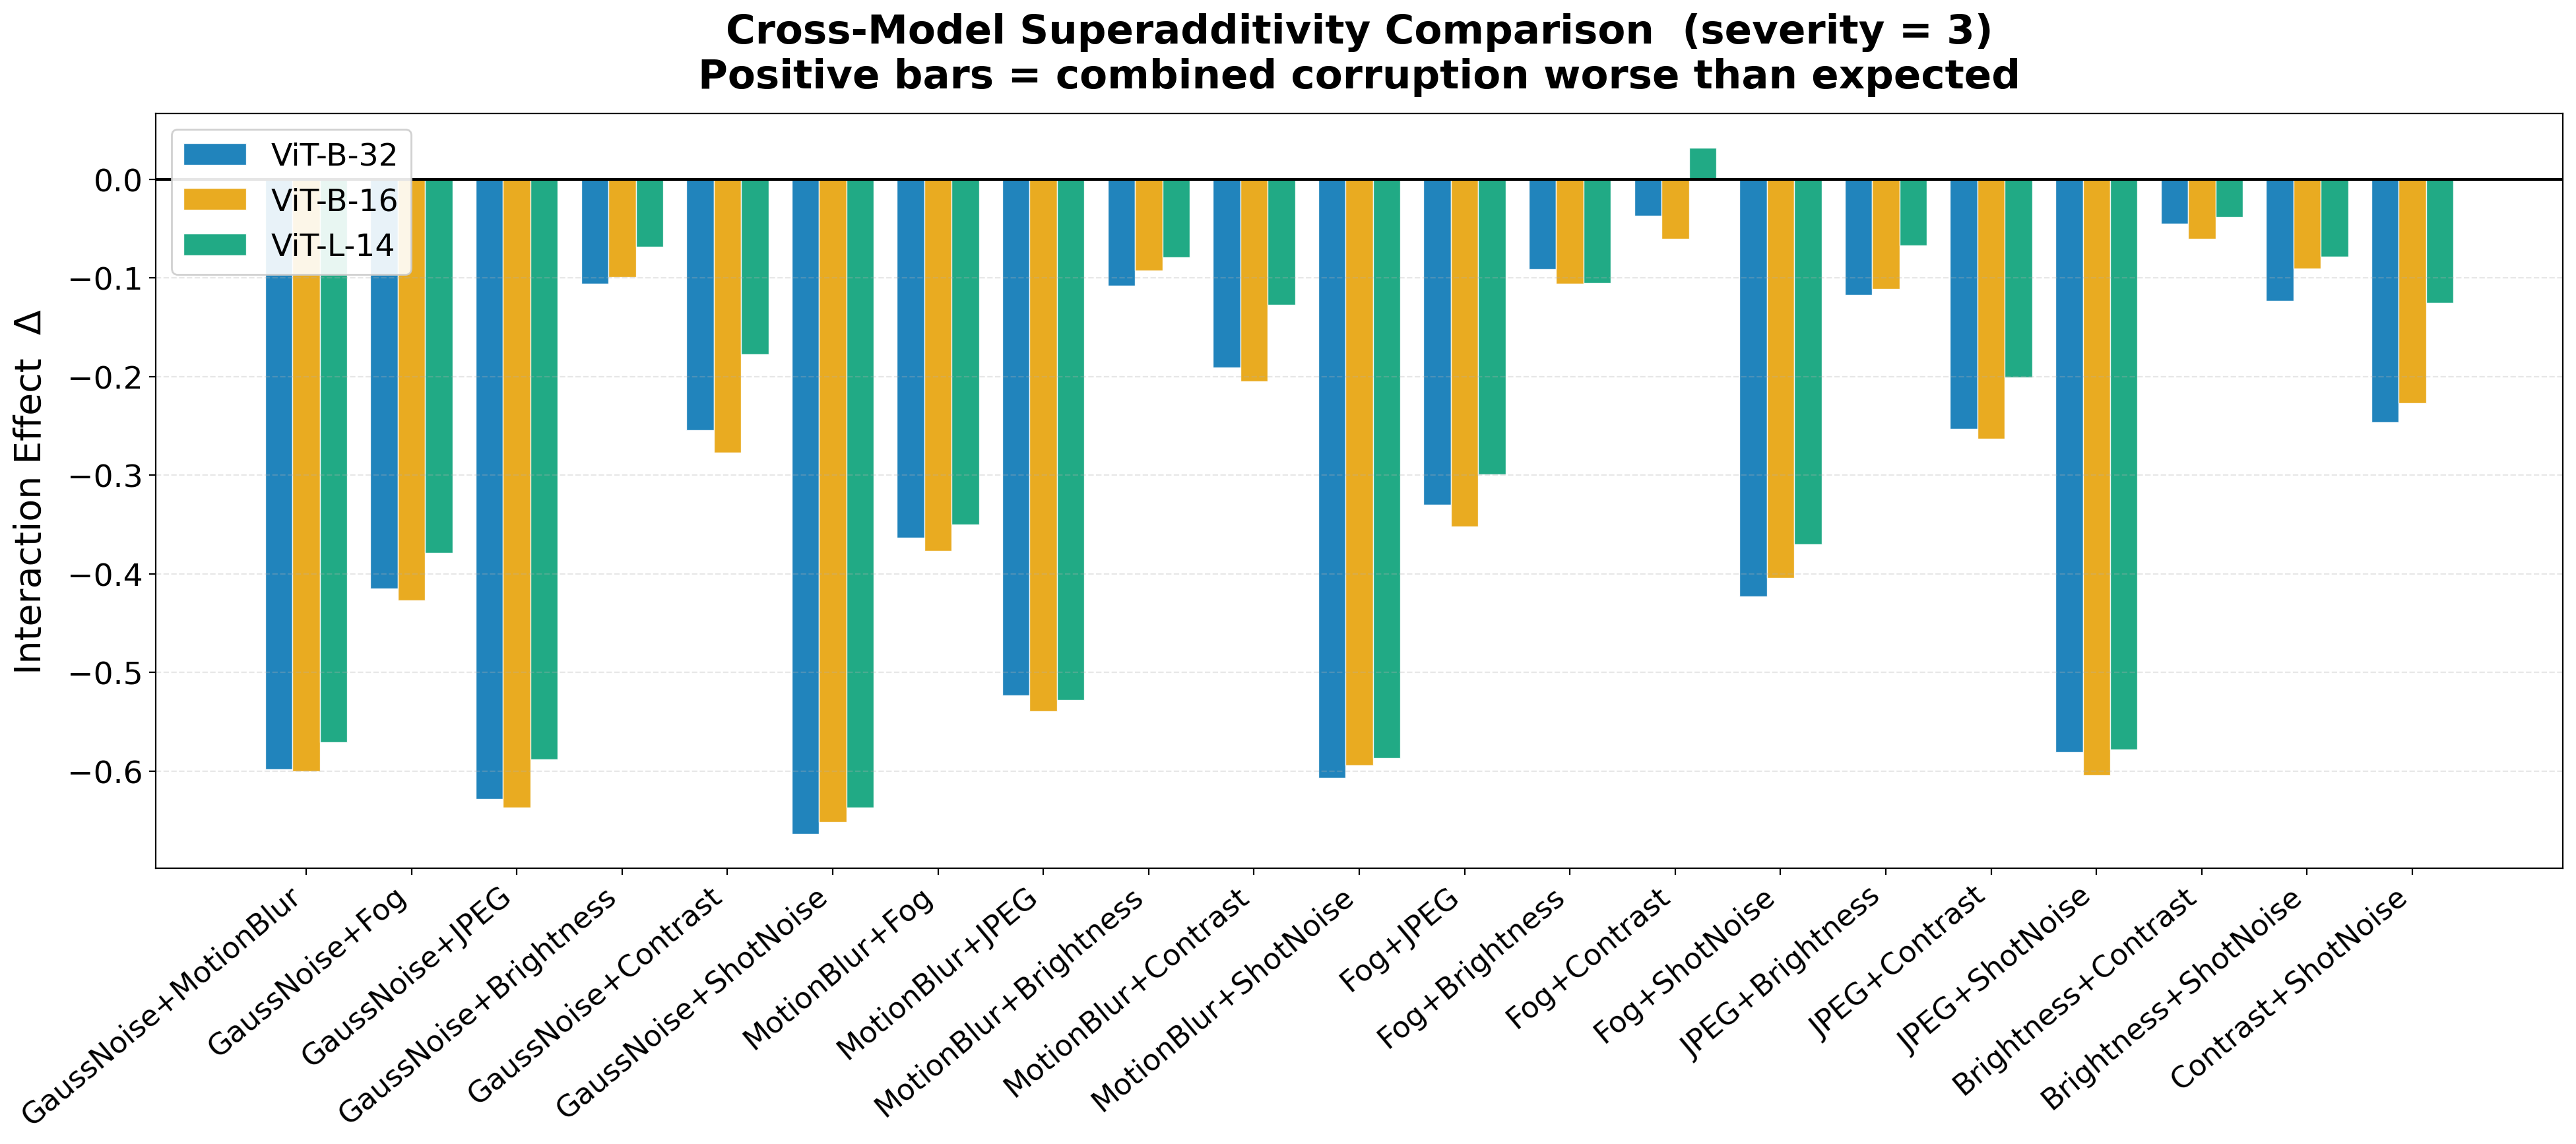
\includegraphics[width=\textwidth]{cross_model_superadditivity.png}
  \caption{
    Cross-model comparison of interaction effects
    $\cI$ (\cref{eq:interaction}) for all 21~corruption
    pairs at severity $s=3$.
    Grouped bars show ViT-B/32 (blue), ViT-B/16
    (orange), and ViT-L/14 (green).
    Positive values indicate superadditive pairs.
    ViT-L/14 consistently shows the largest positive
    interactions, confirming that model scale amplifies
    superadditivity (\cref{sec:rq2}).
  }
  \label{fig:crossmodel}
\end{figure*}

\paragraph{Corruption hierarchy.}
Averaged across all models at $s=3$, the
robustness ranking is:
\begin{table}[h]
\caption{Single-corruption robustness ranking (averaged across
  all models, severity $s=3$). Higher rank = more robust.}
\label{tab:ranking}
\centering
\small
\begin{tabular}{clc}
\toprule
\textbf{Rank} & \textbf{Corruption} & \textbf{Avg.\ Top-1 ($s{=}3$)} \\
\midrule
1 & \texttt{brightness}        & 0.668 \\
2 & \texttt{contrast}          & 0.522 \\
3 & \texttt{fog}               & 0.317 \\
4 & \texttt{jpeg\_compression} & 0.170 \\
5 & \texttt{motion\_blur}      & 0.126 \\
6 & \texttt{gaussian\_noise}   & 0.097 \\
7 & \texttt{shot\_noise}       & 0.089 \\
\bottomrule
\end{tabular}
\end{table}
This ranking is \textbf{invariant across all three
architectures}, suggesting a structural property of
patch-based encoders rather than a parametric one.
\cref{fig:radar} visualises the robustness profile
of each model as a radar chart, making the corruption
hierarchy and cross-model differences immediately
apparent.

\begin{figure}[t]
  \centering
  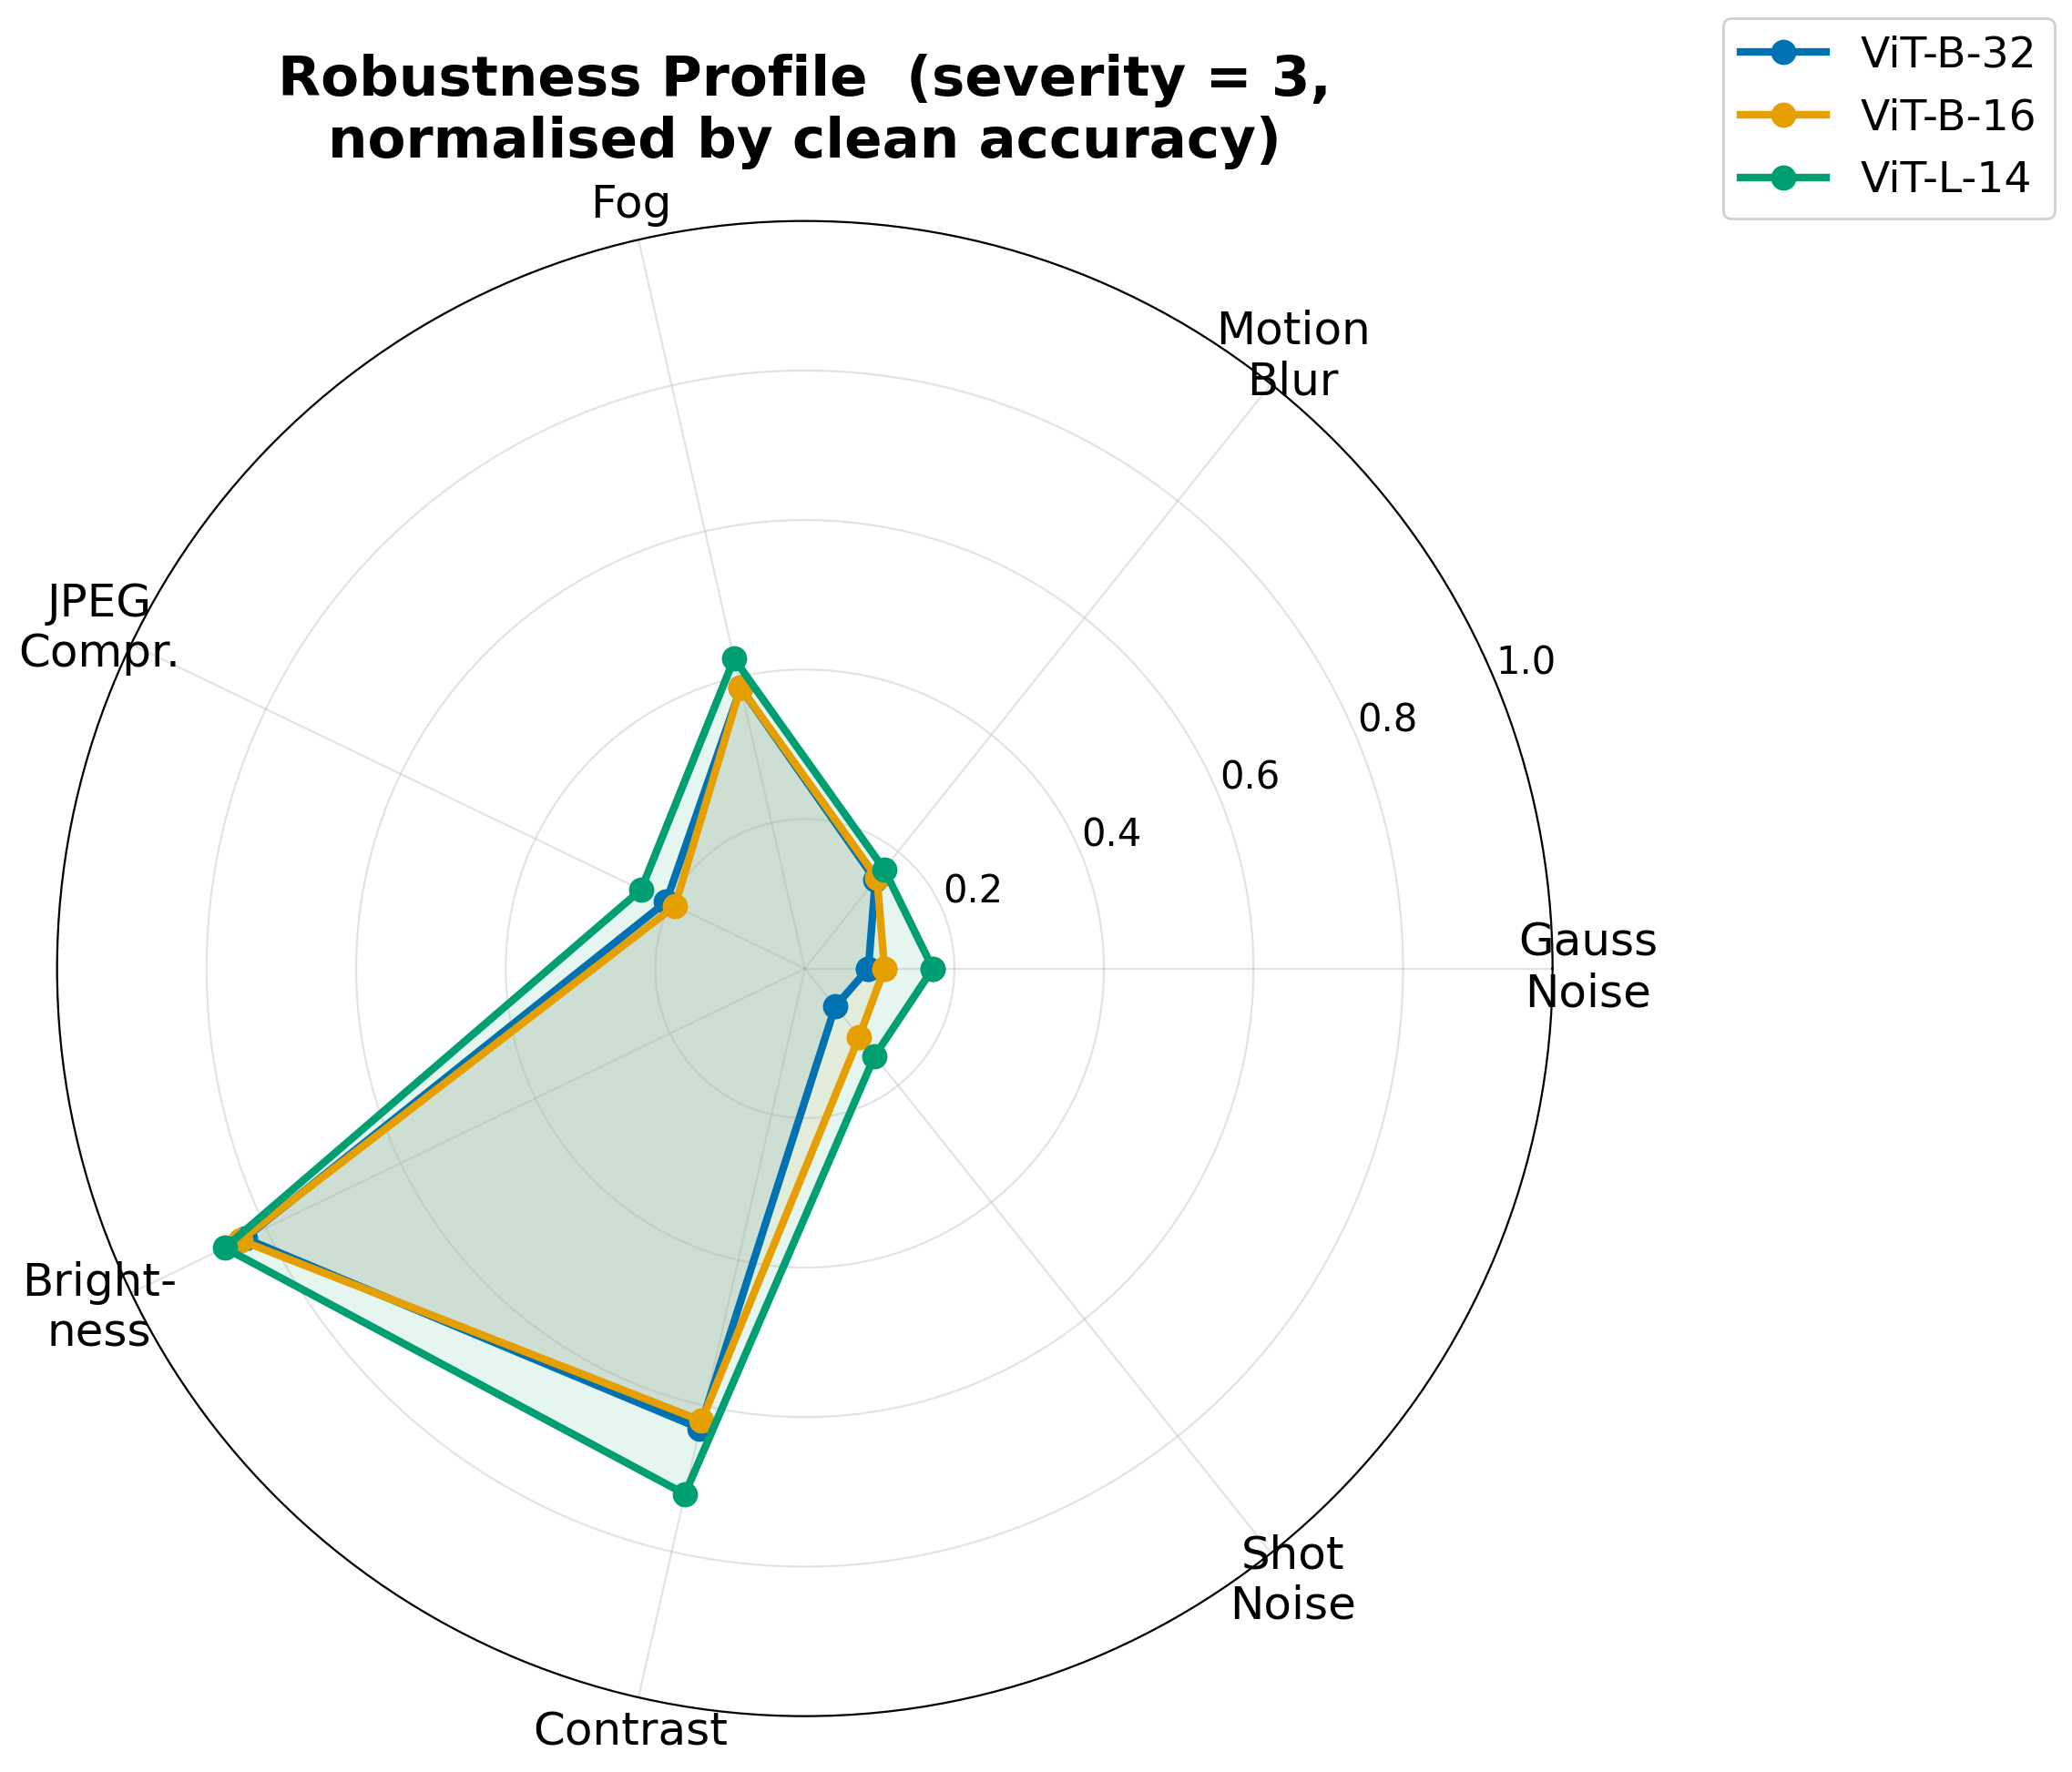
\includegraphics[width=\linewidth]{radar_robustness.png}
  \caption{
    Robustness radar chart for all three models at
    severity $s=3$, normalised by clean accuracy.
    Each axis represents one corruption type; larger
    enclosed area indicates higher robustness.
    All models share the same profile shape,
    confirming that the corruption hierarchy is
    architecture-invariant.
    ViT-L/14 (green) occupies the largest area,
    consistent with its higher clean accuracy.
  }
  \label{fig:radar}
\end{figure}

\paragraph{Patch-size trade-off.}
ViT-B/16 outperforms ViT-B/32 on
\texttt{gaussian\_noise} at $s=1$
\paragraph{Patch-size trade-off.}
ViT-B/16 outperforms ViT-B/32 on
\texttt{gaussian\_noise} at $s=1$
($0.341$ vs.\ $0.276$, $+6.5$~pp) but
\emph{underperforms} on \texttt{jpeg\_compression}
($0.279$ vs.\ $0.290$, $-1.1$~pp).
Smaller patches provide finer spatial granularity
aiding noise recovery, but JPEG artifacts manifest
as high-frequency ringing that is more disruptive
to fine-grained patch embeddings.

\noindent\textbf{Finding 2:}
\textit{Patch size creates a noise/JPEG trade-off:
ViT-B/16 is more robust to noise but less robust
to compression than ViT-B/32.}

% -------------------------------------------------------
% RQ4 — Order sensitivity (Finding #6)
% -------------------------------------------------------
\subsection{RQ4: Does Corruption Order Matter?}
\label{sec:rq4}

% -------------------------------------------------------
% TABLE 4 — Ablation: order sensitivity
% -------------------------------------------------------
\begin{table}[t]
\caption{
  Order sensitivity of top superadditive pairs on
  ViT-B/32, severity $s=1$.
  $\cI$~= interaction effect (\cref{eq:interaction}).
  $\Delta_{\mathrm{order}}$~= $|$acc$(c_1{\to}c_2)
  -$ acc$(c_2{\to}c_1)|$.
  Large values indicate worst-case evaluation
  requires testing \emph{both} orders.
}
\label{tab:ablation}
\centering
\small
\setlength{\tabcolsep}{3pt}
\begin{tabular}{lccccc}
\toprule
\textbf{Pair}
  & \textbf{$c_1{\to}c_2$}
  & \textbf{$c_2{\to}c_1$}
  & $\Delta_{\mathrm{order}}$
  & $\cI_{c_1 \to c_2}$
  & \textbf{Verdict} \\
\midrule
contrast+shot & 0.039 & 0.214 & 0.175
  & +0.107 & Sensitive \\
fog+contrast  & 0.356 & 0.146 & 0.210
  & +0.052 & Sensitive \\
fog+shot      & 0.021 & 0.126 & 0.105
  & $-$0.010 & Sensitive \\
blur+fog      & 0.122 & 0.173 & 0.051
  & +0.065 & Sensitive \\
blur+contrast & 0.259 & 0.266 & 0.007
  & +0.063 & \textbf{Invariant} \\
\bottomrule
\end{tabular}
\end{table}

\cref{tab:ablation} shows that 4 of~5 top pairs
exhibit significant order sensitivity
($\Delta_{\mathrm{order}} > 0.01$).
The most extreme case is \texttt{fog\,+\,contrast}:
applying contrast \emph{after} fog yields $0.356$
accuracy, while reversing the order collapses it
to $0.146$---a gap of $0.210$.

We hypothesise two mechanisms:
\begin{itemize}[leftmargin=*]
  \item \textbf{Amplification.} When a structural
        corruption (\texttt{contrast}, \texttt{fog})
        is applied first, it removes semantic anchors
        that would otherwise limit damage from
        subsequent noise.
  \item \textbf{Partial cancellation.} When noise is
        applied first, a subsequent contrast
        adjustment can inadvertently compress the
        noise range, reducing its perceptual impact.
\end{itemize}

\noindent\textbf{Finding 3:}
\textit{Worst-case evaluation must consider both
orders of each pair.
Fixed-order protocols underestimate worst-case
degradation by up to 0.21 in absolute accuracy.}

% -------------------------------------------------------
% FIGURE 2 — Heatmaps
% -------------------------------------------------------
\begin{figure*}[t]
  \centering
  \begin{subfigure}[b]{0.32\textwidth}
    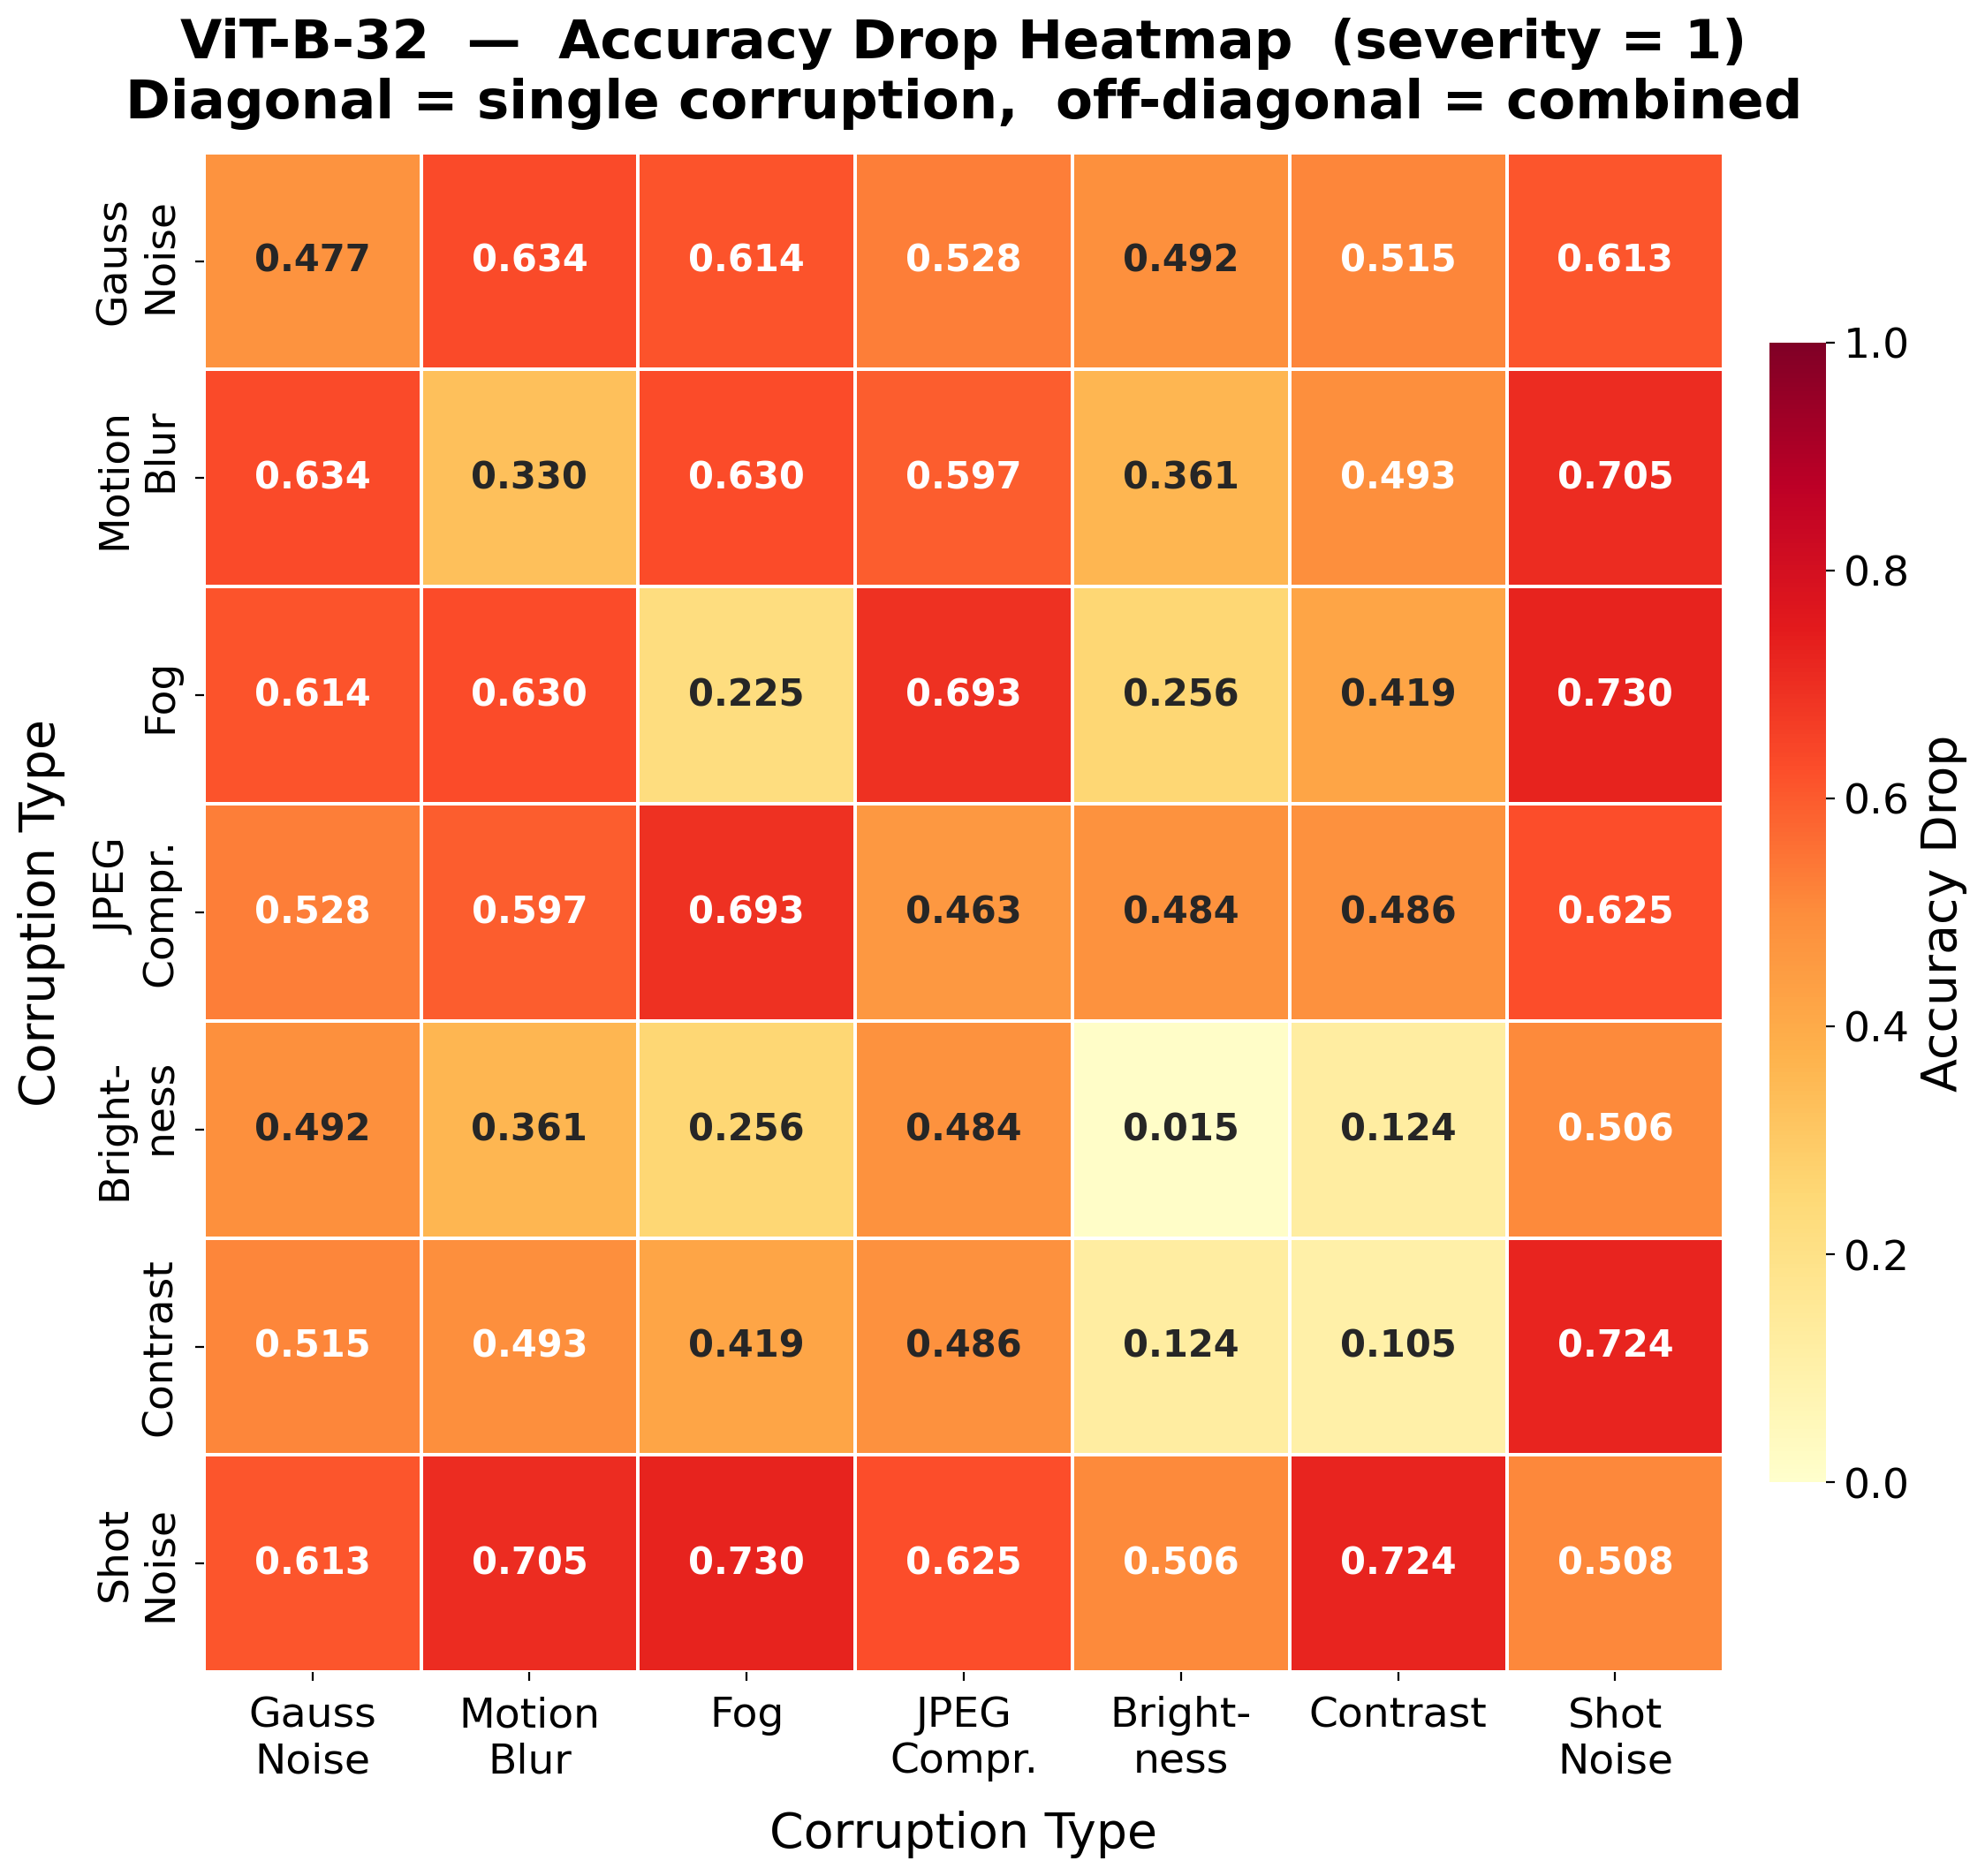
\includegraphics[width=\textwidth]{heatmap_ViT-B-32_s1.png}
    \caption{ViT-B/32, $s=1$}
  \end{subfigure}
  \hfill
  \begin{subfigure}[b]{0.32\textwidth}
    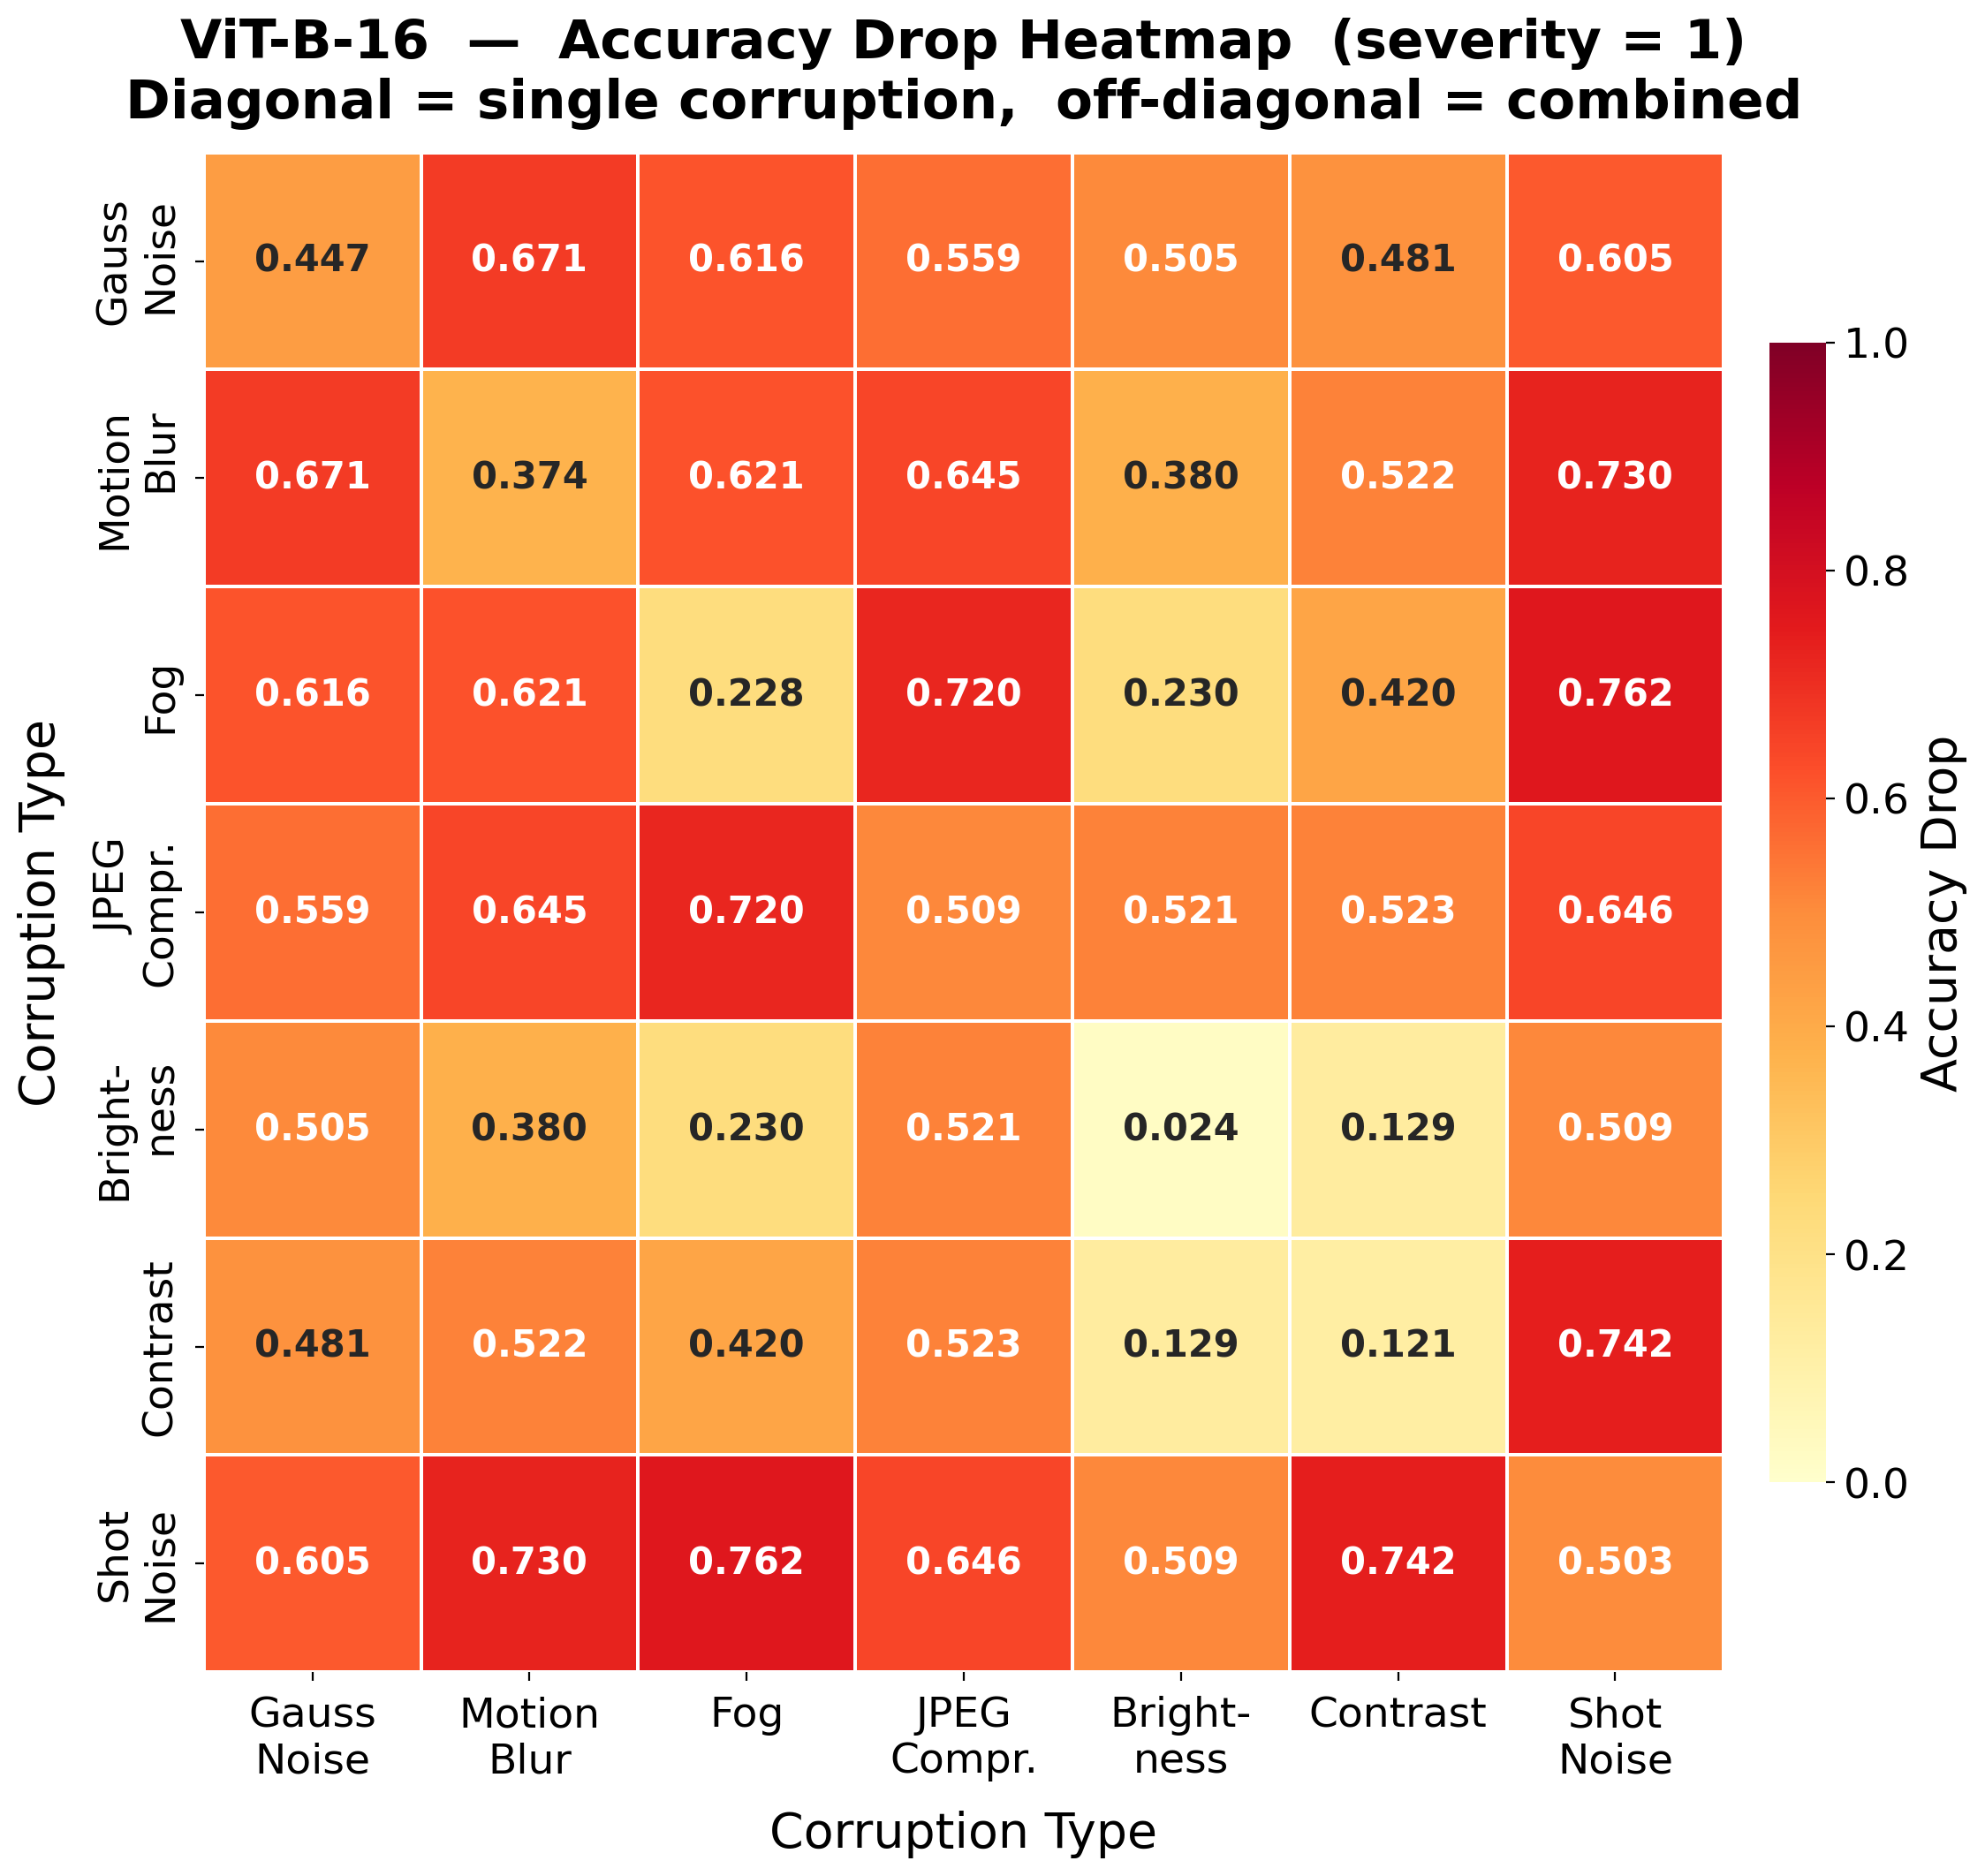
\includegraphics[width=\textwidth]{heatmap_ViT-B-16_s1.png}
    \caption{ViT-B/16, $s=1$}
  \end{subfigure}
  \hfill
  \begin{subfigure}[b]{0.32\textwidth}
    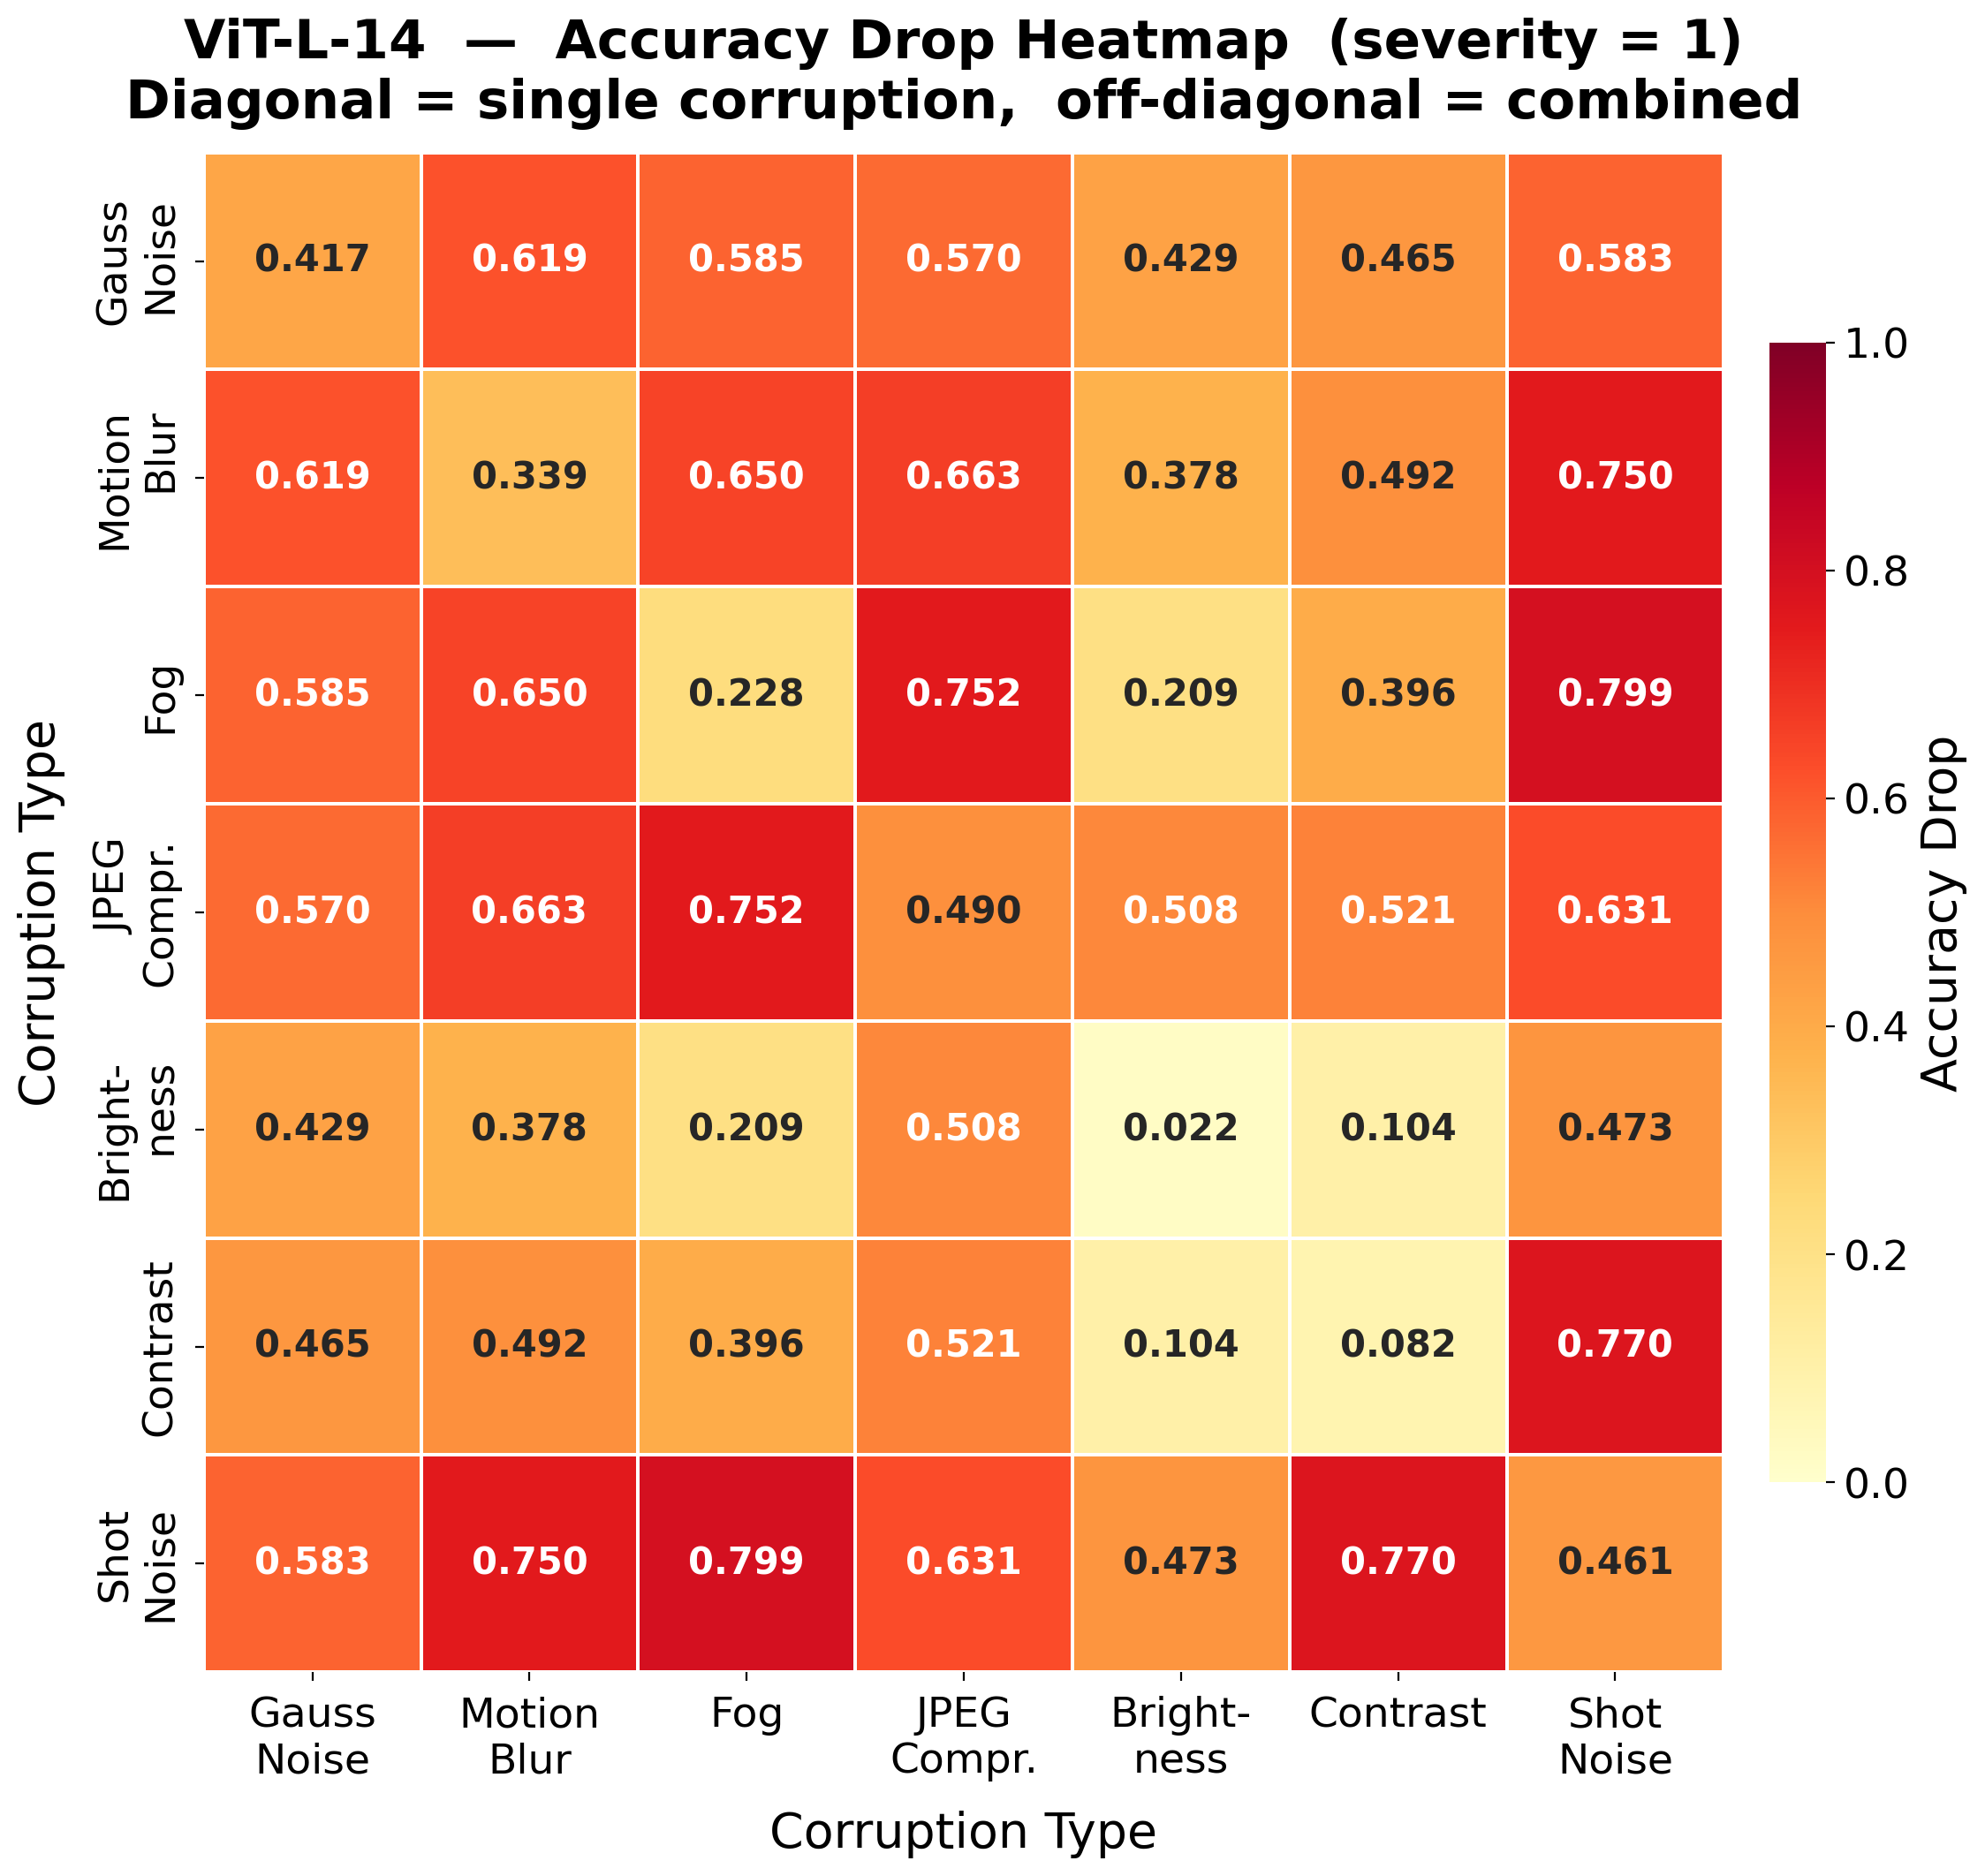
\includegraphics[width=\textwidth]{heatmap_ViT-L-14_s1.png}
    \caption{ViT-L/14, $s=1$}
  \end{subfigure}
  \caption{
    Accuracy drop heatmaps for all pairwise corruption
    combinations at severity $s=1$.
    Diagonal = single-corruption drop;
    off-diagonal = combined-corruption drop.
    Darker red indicates more severe degradation.
    The noise-family quadrant (bottom-right) consistently
    shows the worst combined performance across all
    architectures.
  }
  \label{fig:heatmaps}
\end{figure*}

% -------------------------------------------------------
% FIGURE 3 — Severity curves
% -------------------------------------------------------
\begin{figure*}[t]
  \centering
  \begin{subfigure}[b]{0.32\textwidth}
    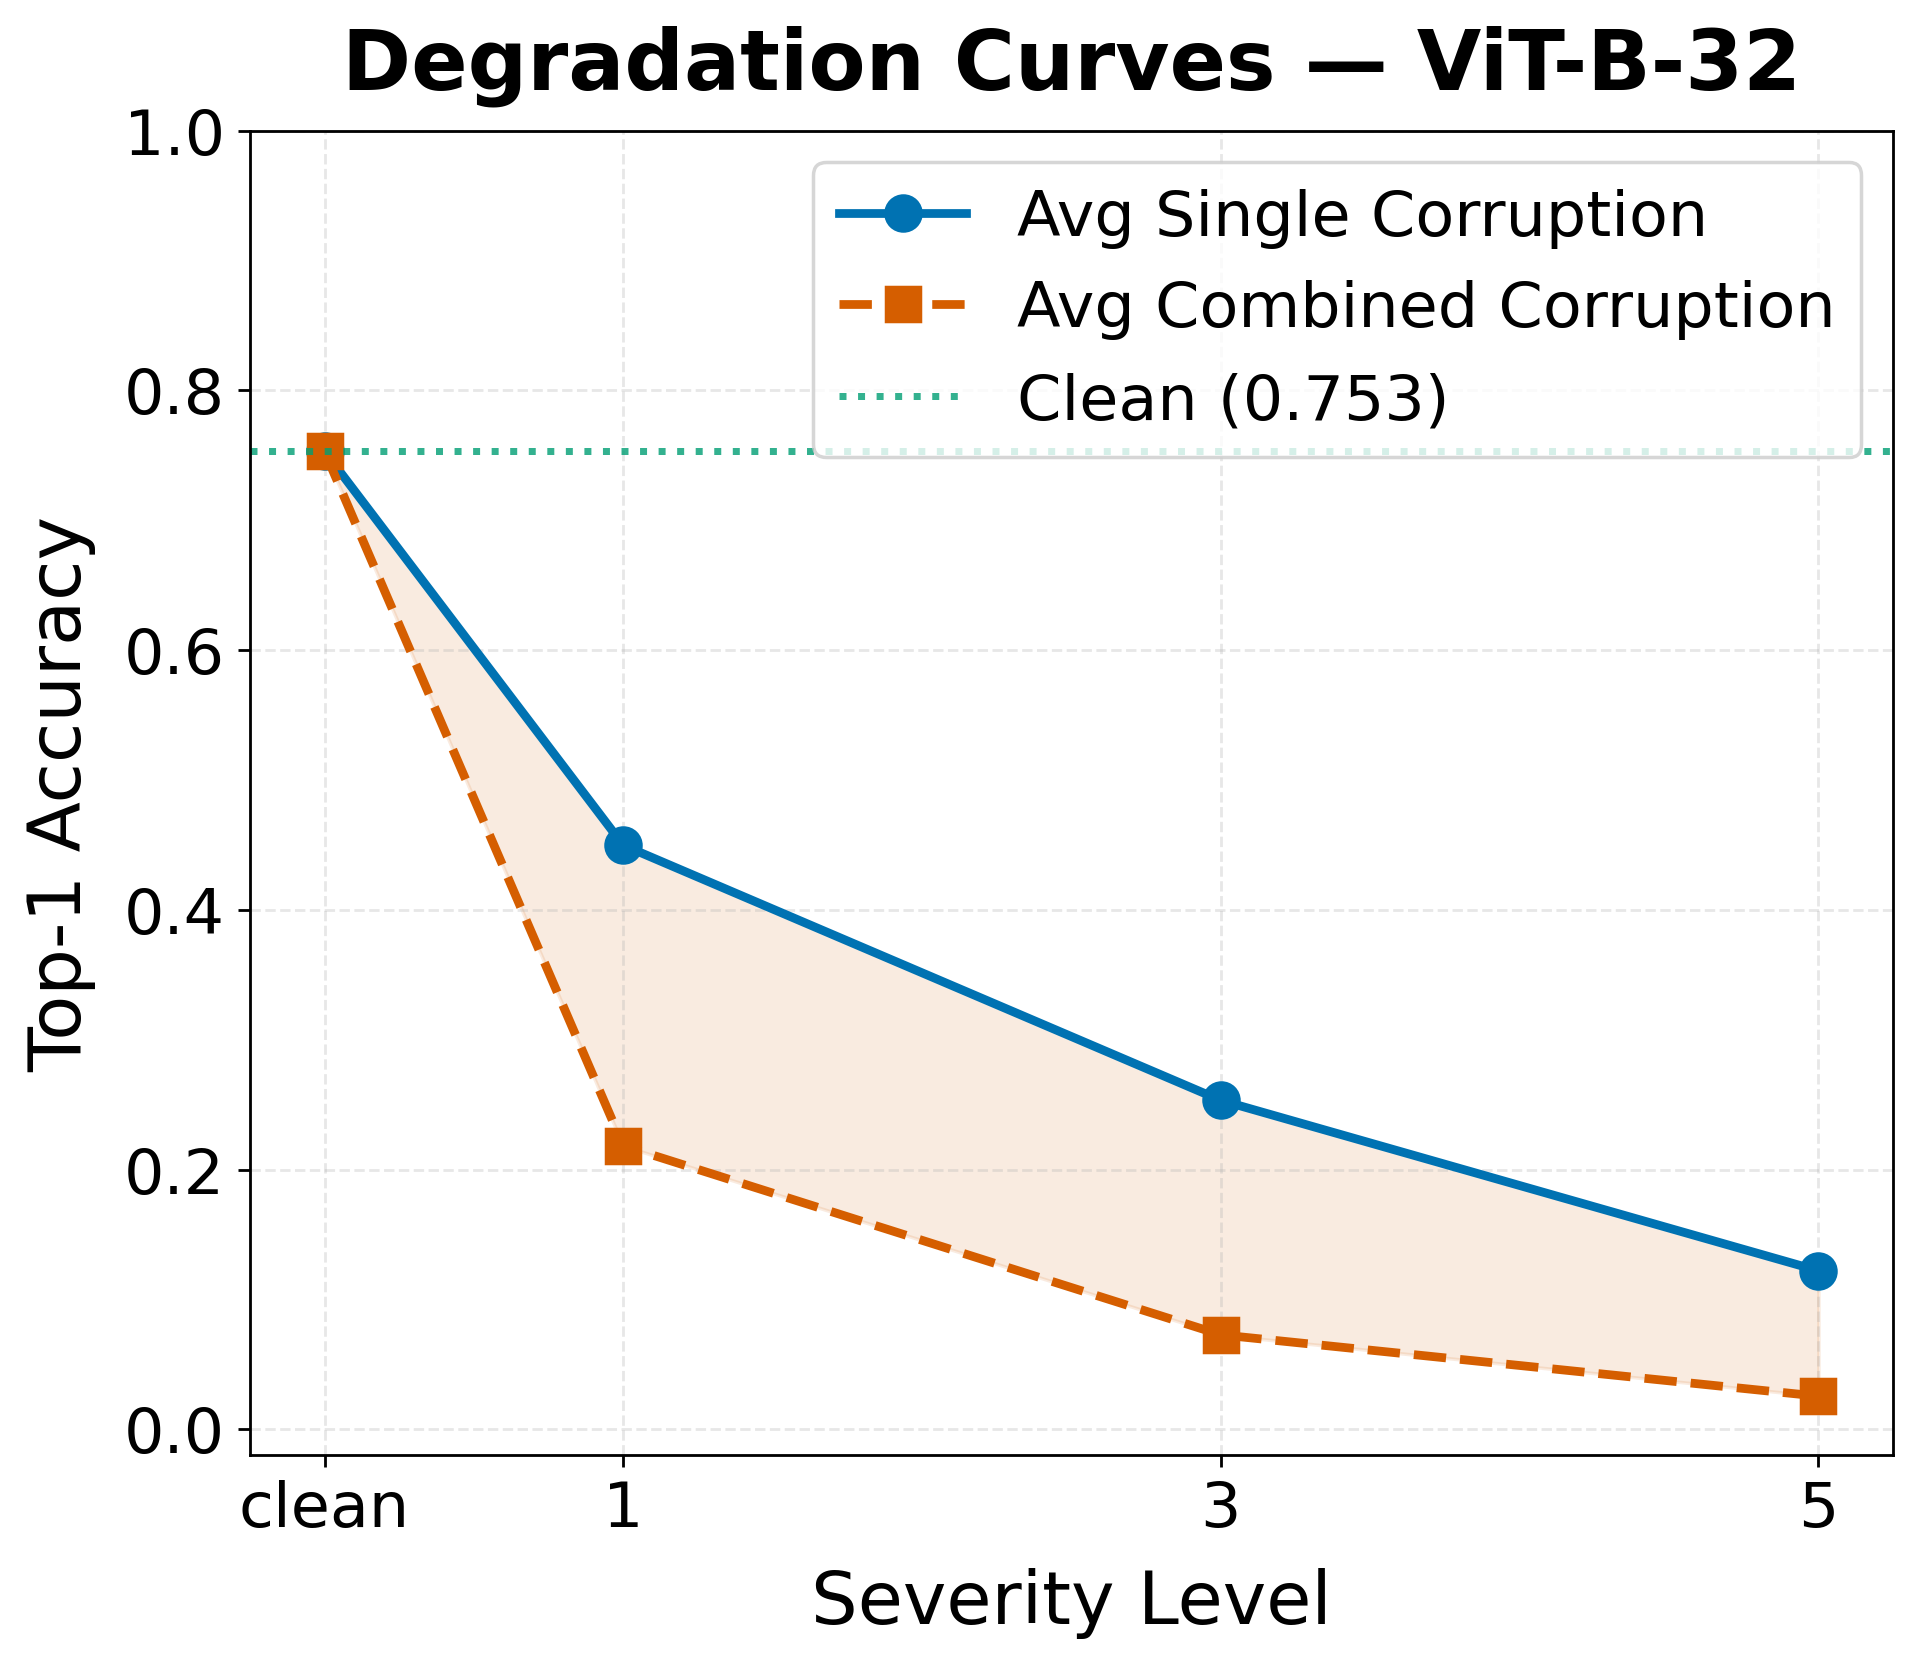
\includegraphics[width=\textwidth]{severity_curves_ViT-B-32.png}
    \caption{ViT-B/32}
  \end{subfigure}
  \hfill
  \begin{subfigure}[b]{0.32\textwidth}
    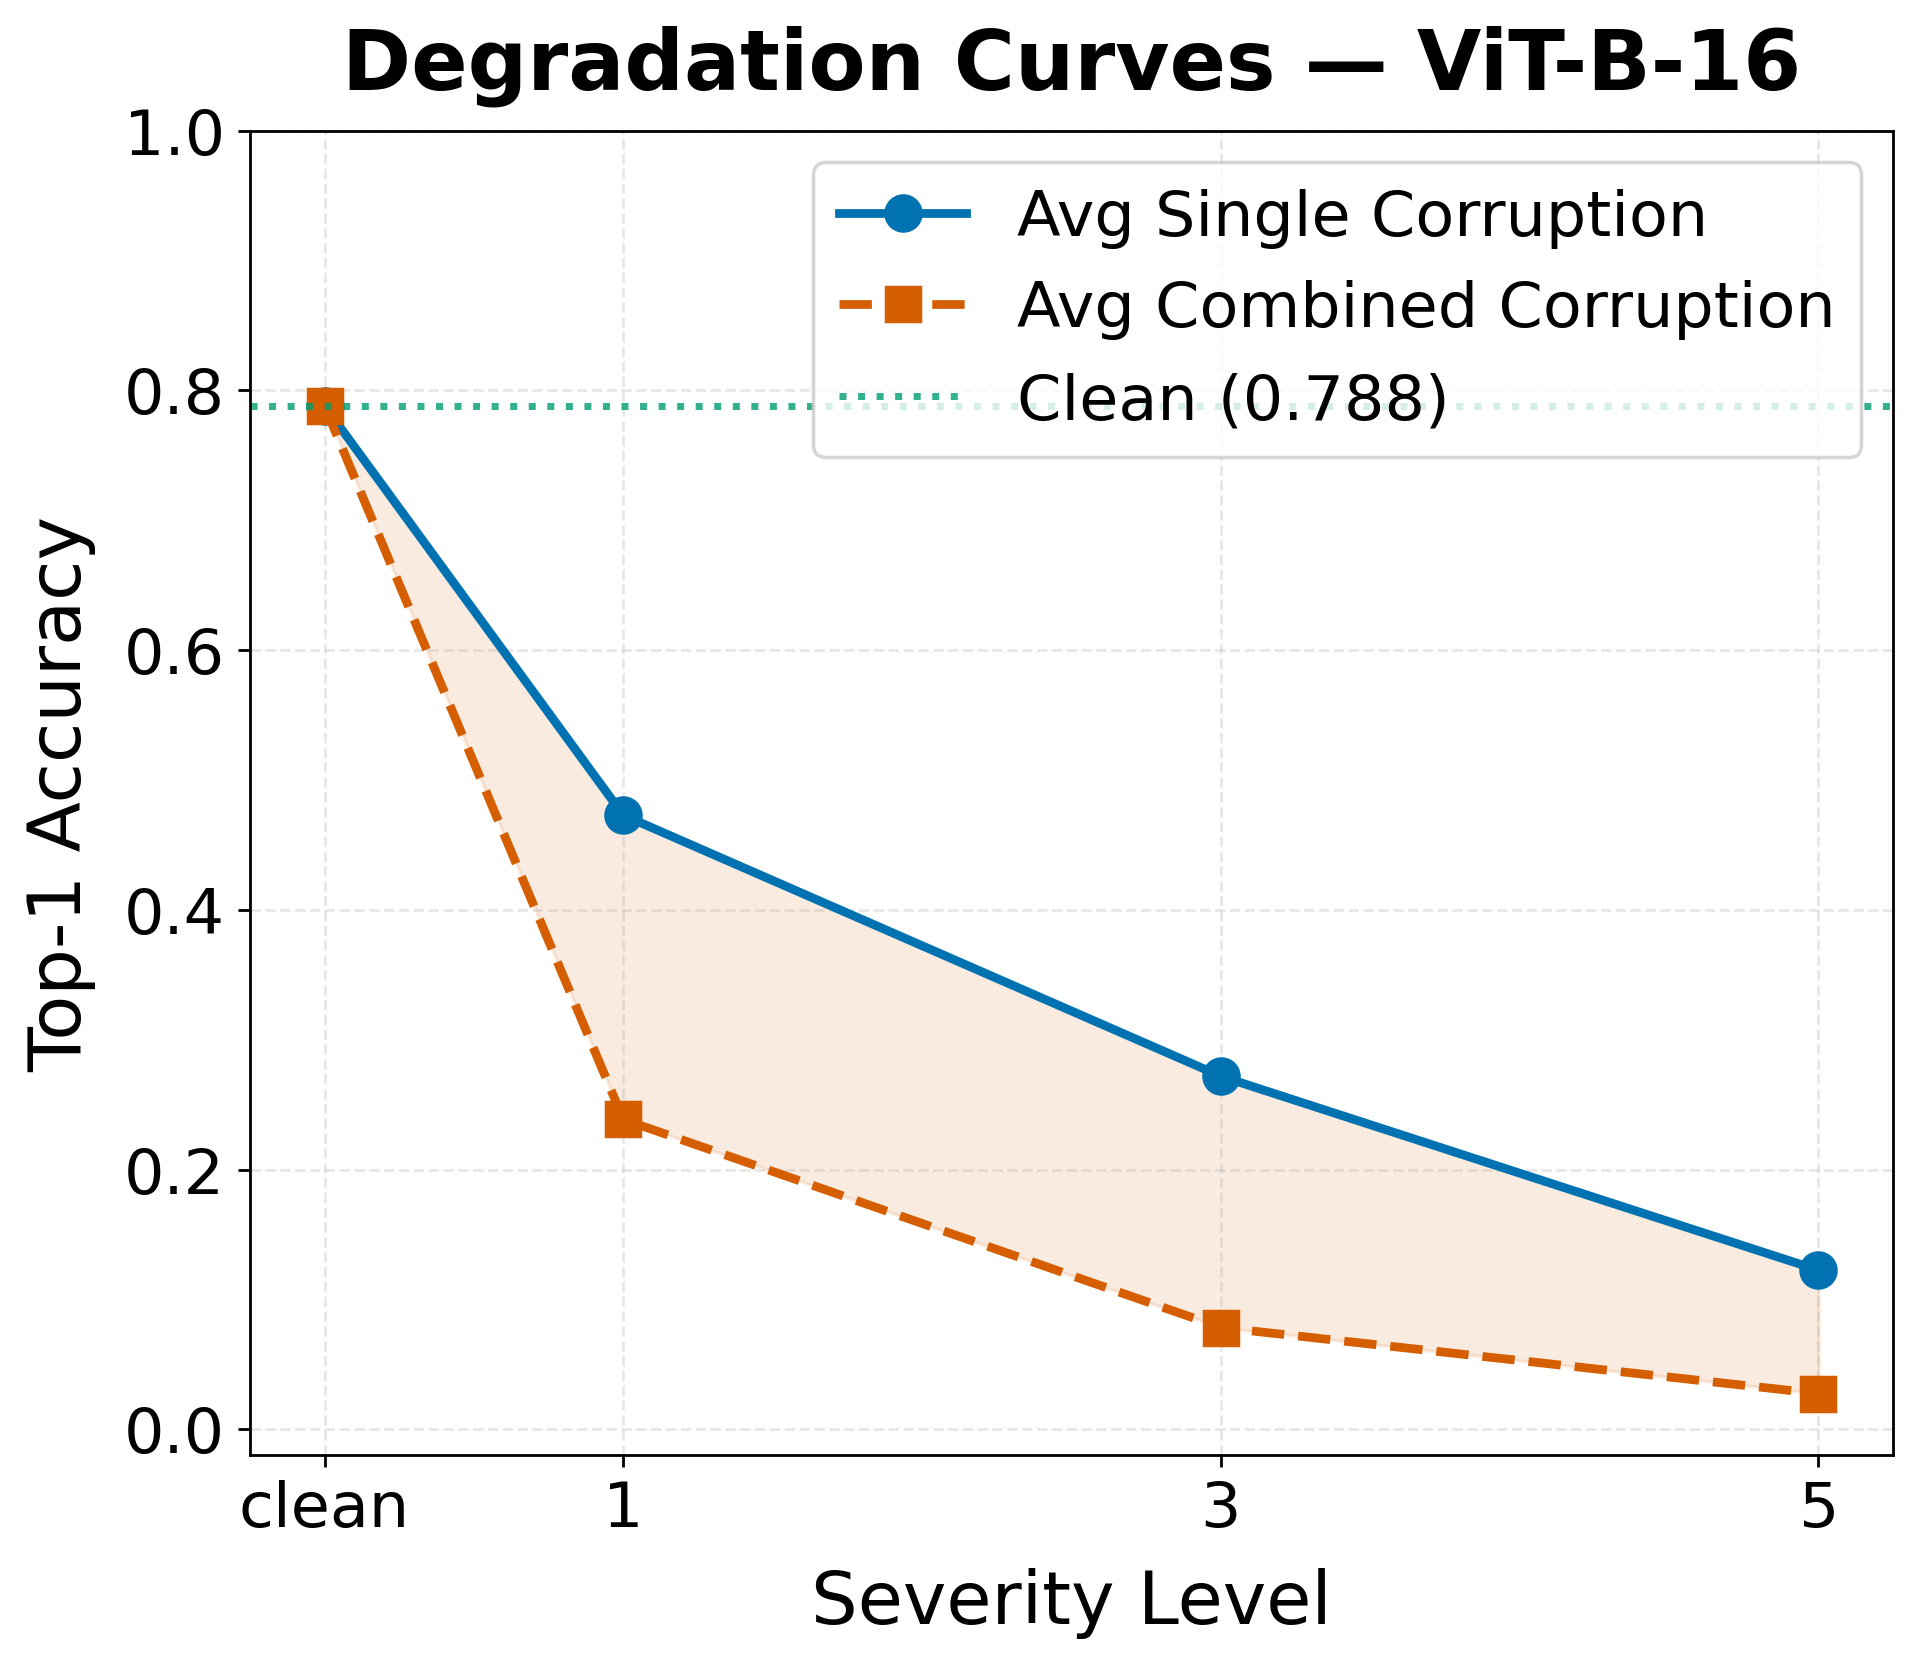
\includegraphics[width=\textwidth]{severity_curves_ViT-B-16.png}
    \caption{ViT-B/16}
  \end{subfigure}
  \hfill
  \begin{subfigure}[b]{0.32\textwidth}
    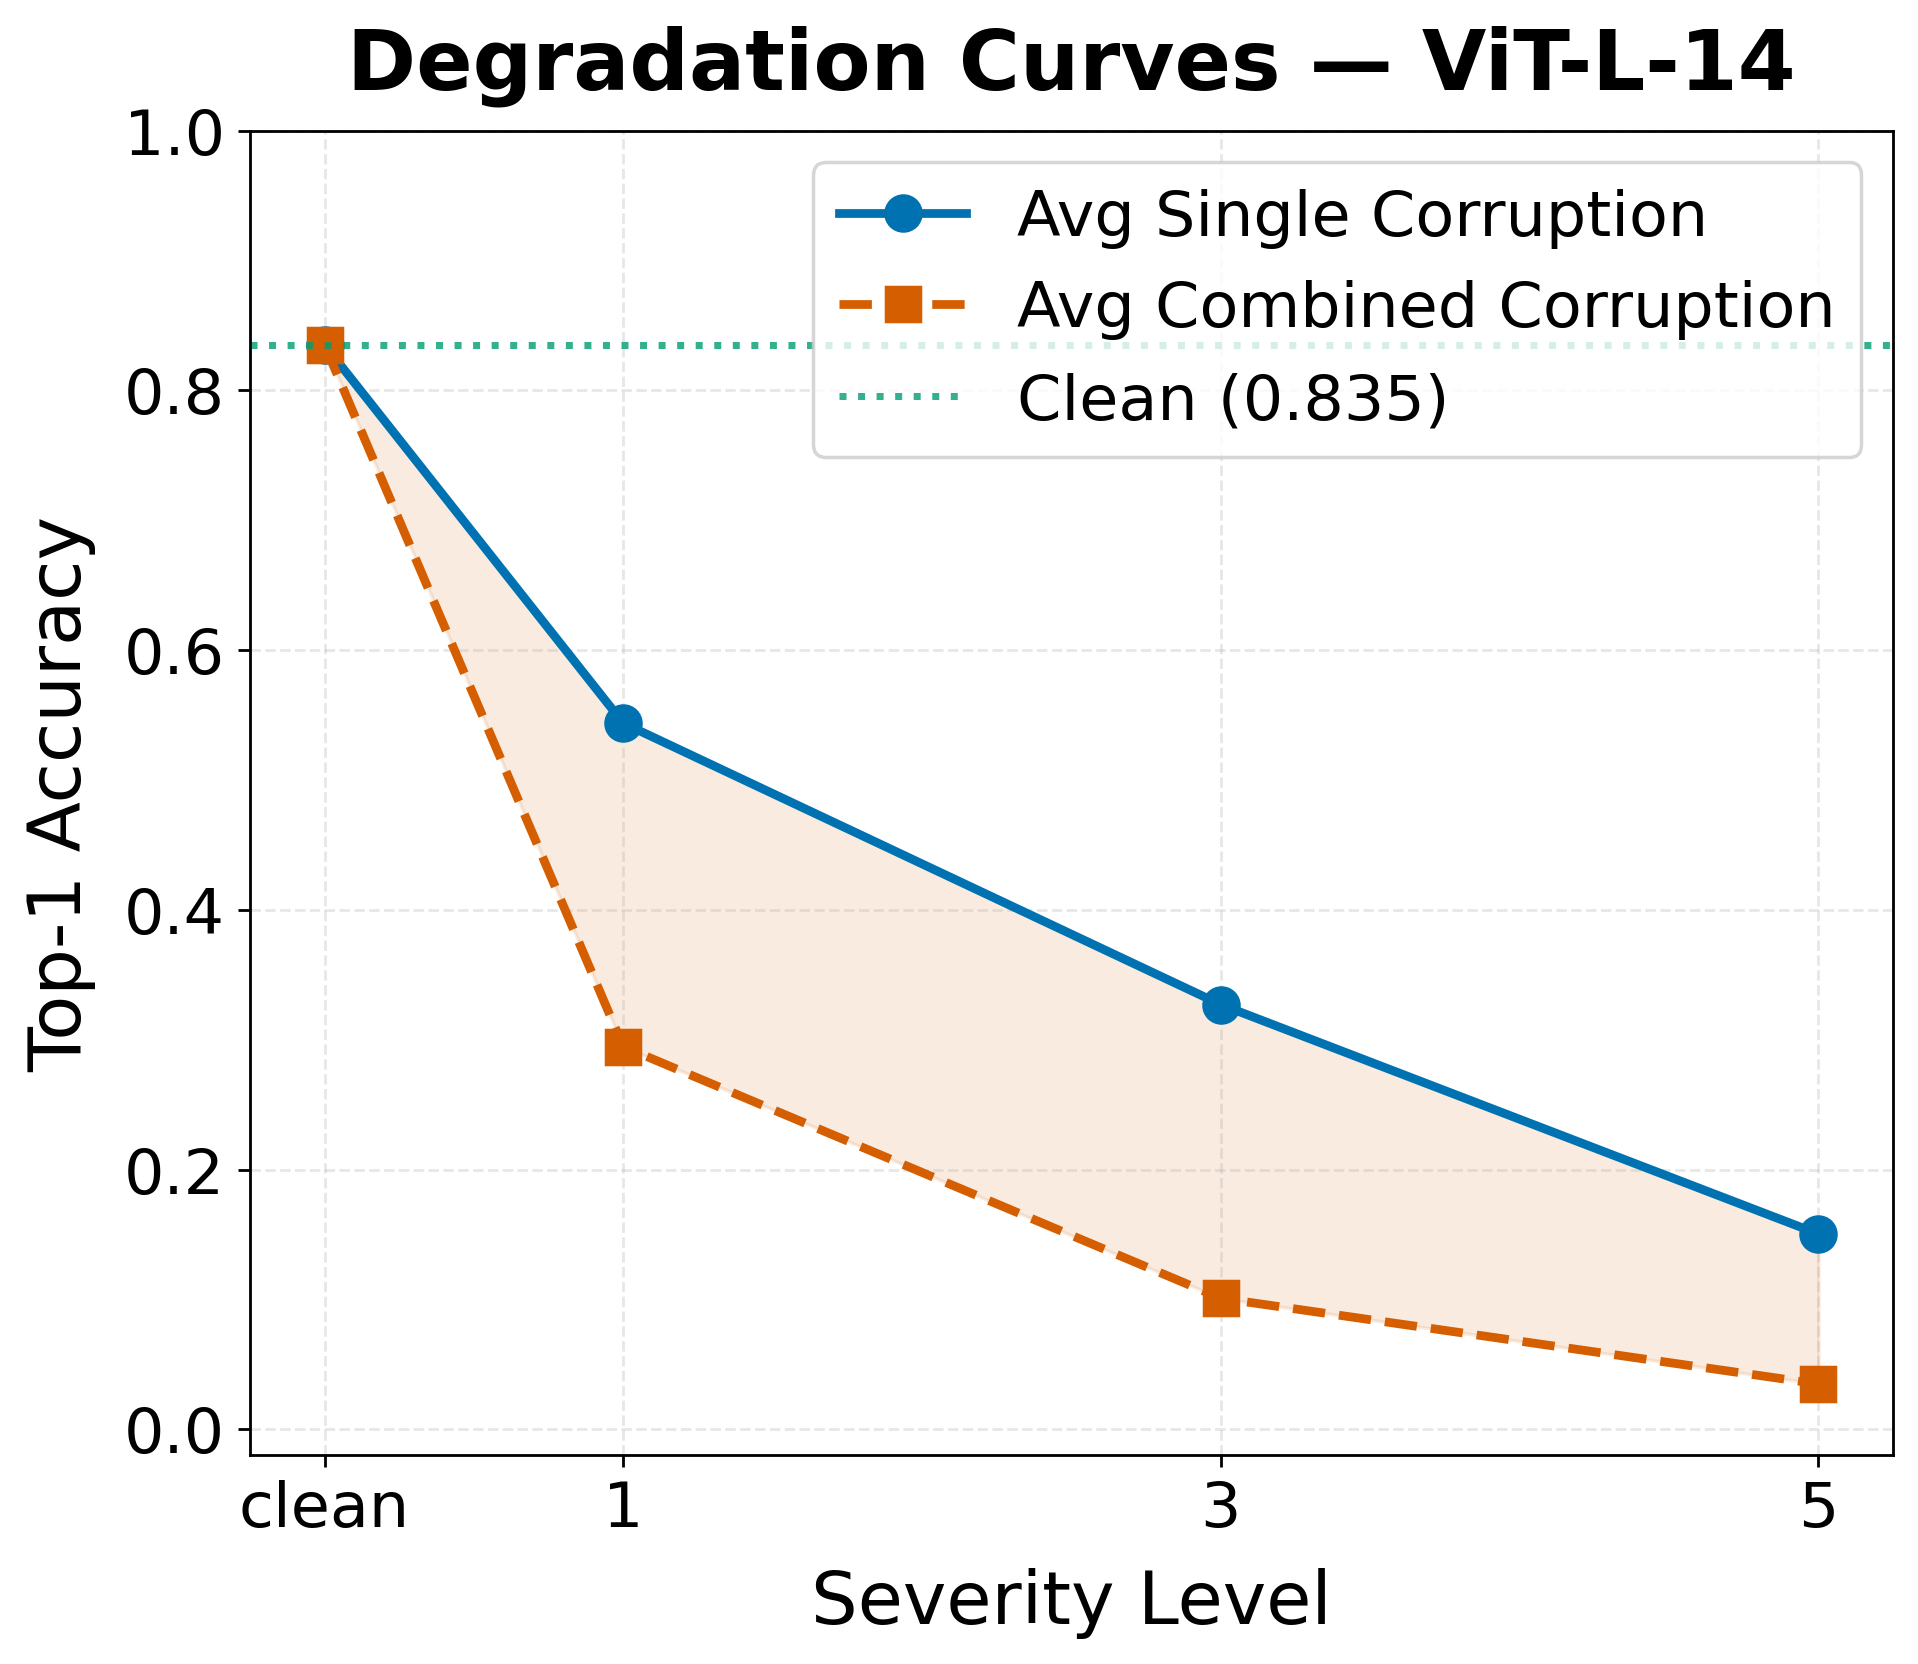
\includegraphics[width=\textwidth]{severity_curves_ViT-L-14.png}
    \caption{ViT-L/14}
  \end{subfigure}
  \caption{
    Average Top-1 accuracy vs.\ severity for single
    corruptions (blue, solid) and combined corruptions
    (red, dashed).
    The gap between curves narrows at high severity,
    illustrating the floor effect (\cref{sec:rq1}).
    Clean accuracy is shown as a green dotted baseline.
  }
  \label{fig:severity}
\end{figure*}

% -------------------------------------------------------
% FIGURE 4 — Superadditivity bars
% -------------------------------------------------------
\begin{figure*}[t]
  \centering

  \begin{subfigure}{\textwidth}
    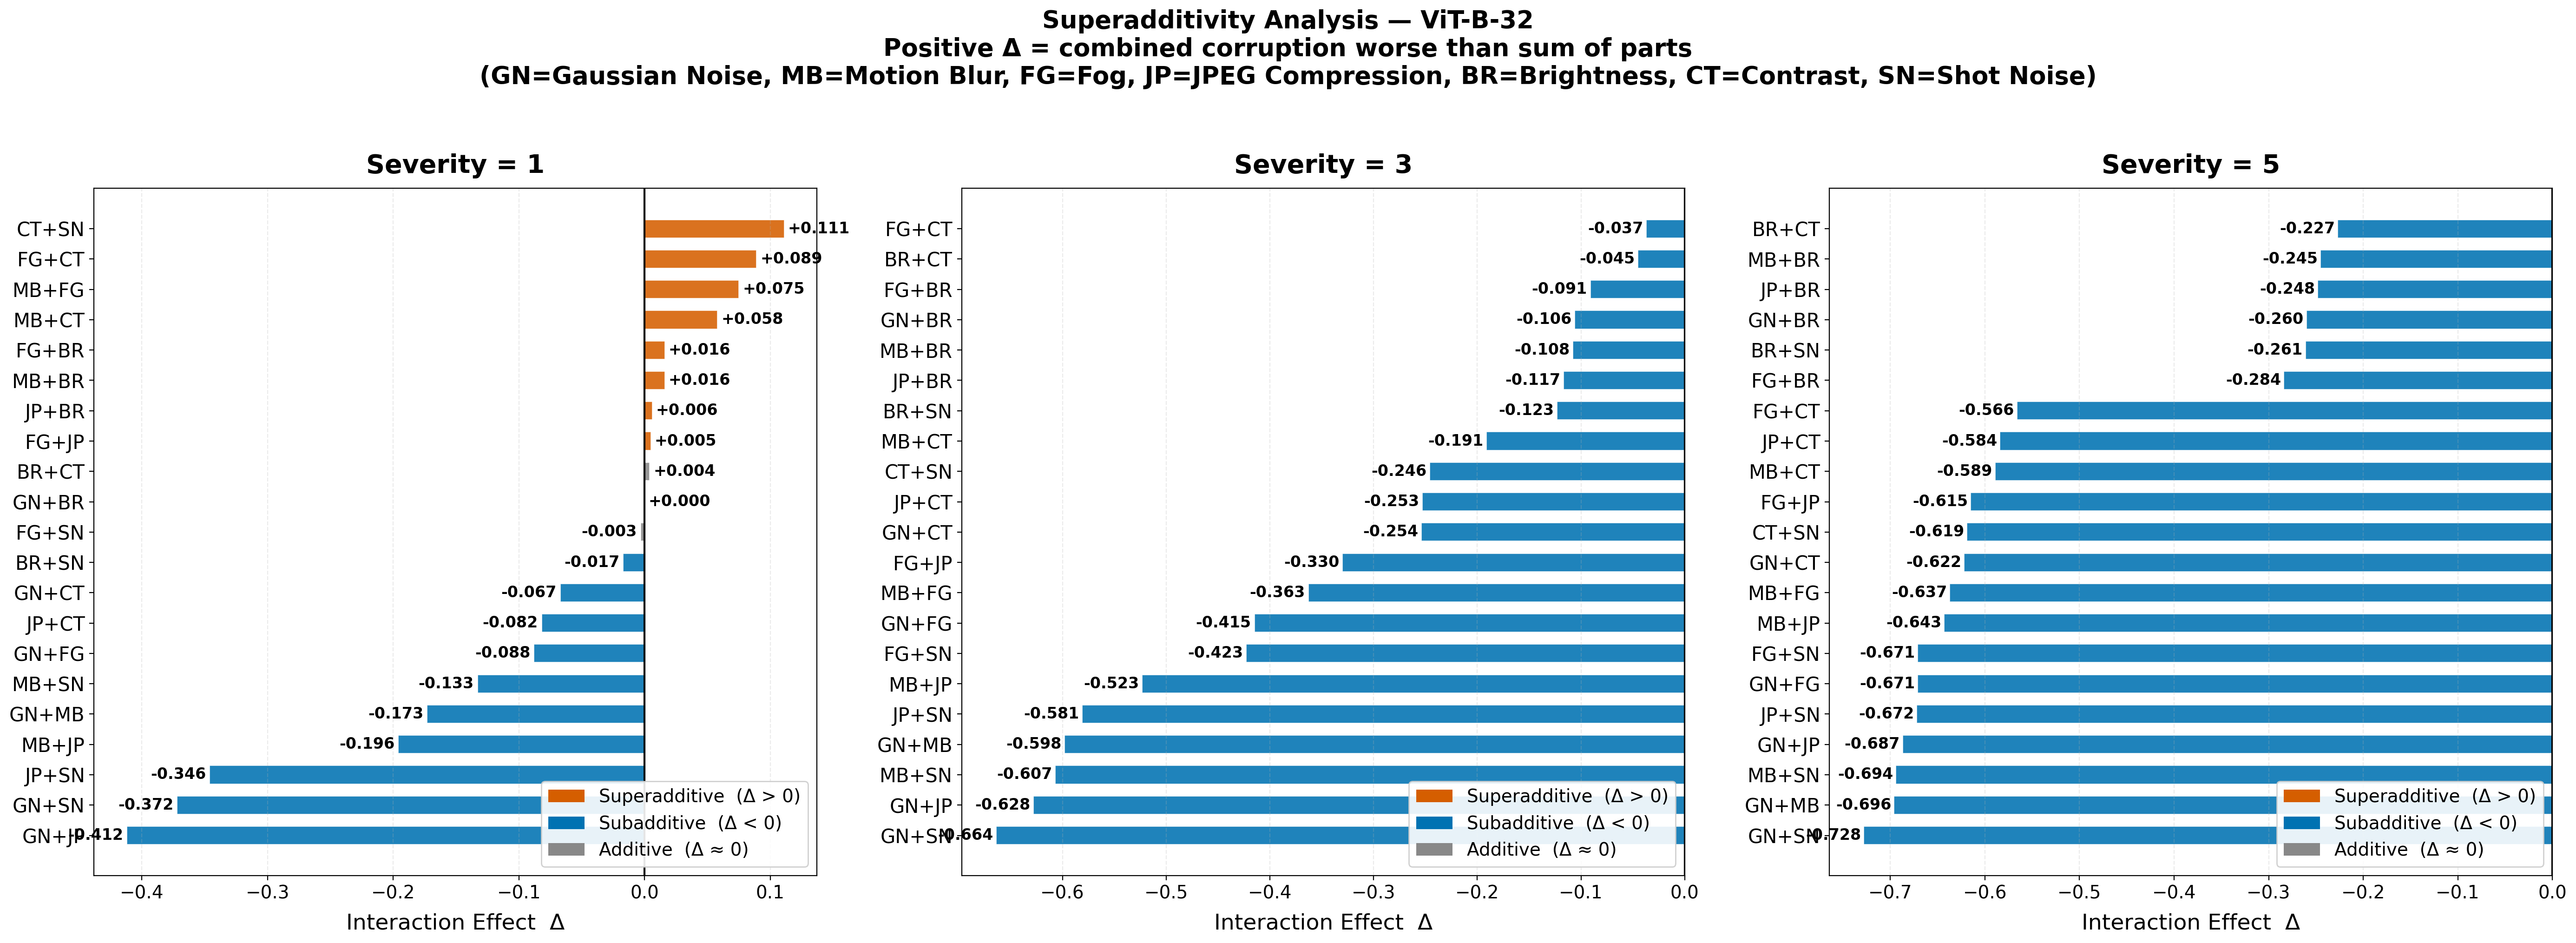
\includegraphics[width=\textwidth]{superadditivity_ViT-B-32.png}
    \caption{ViT-B/32}
  \end{subfigure}

  \vspace{6pt}

  \begin{subfigure}{\textwidth}
    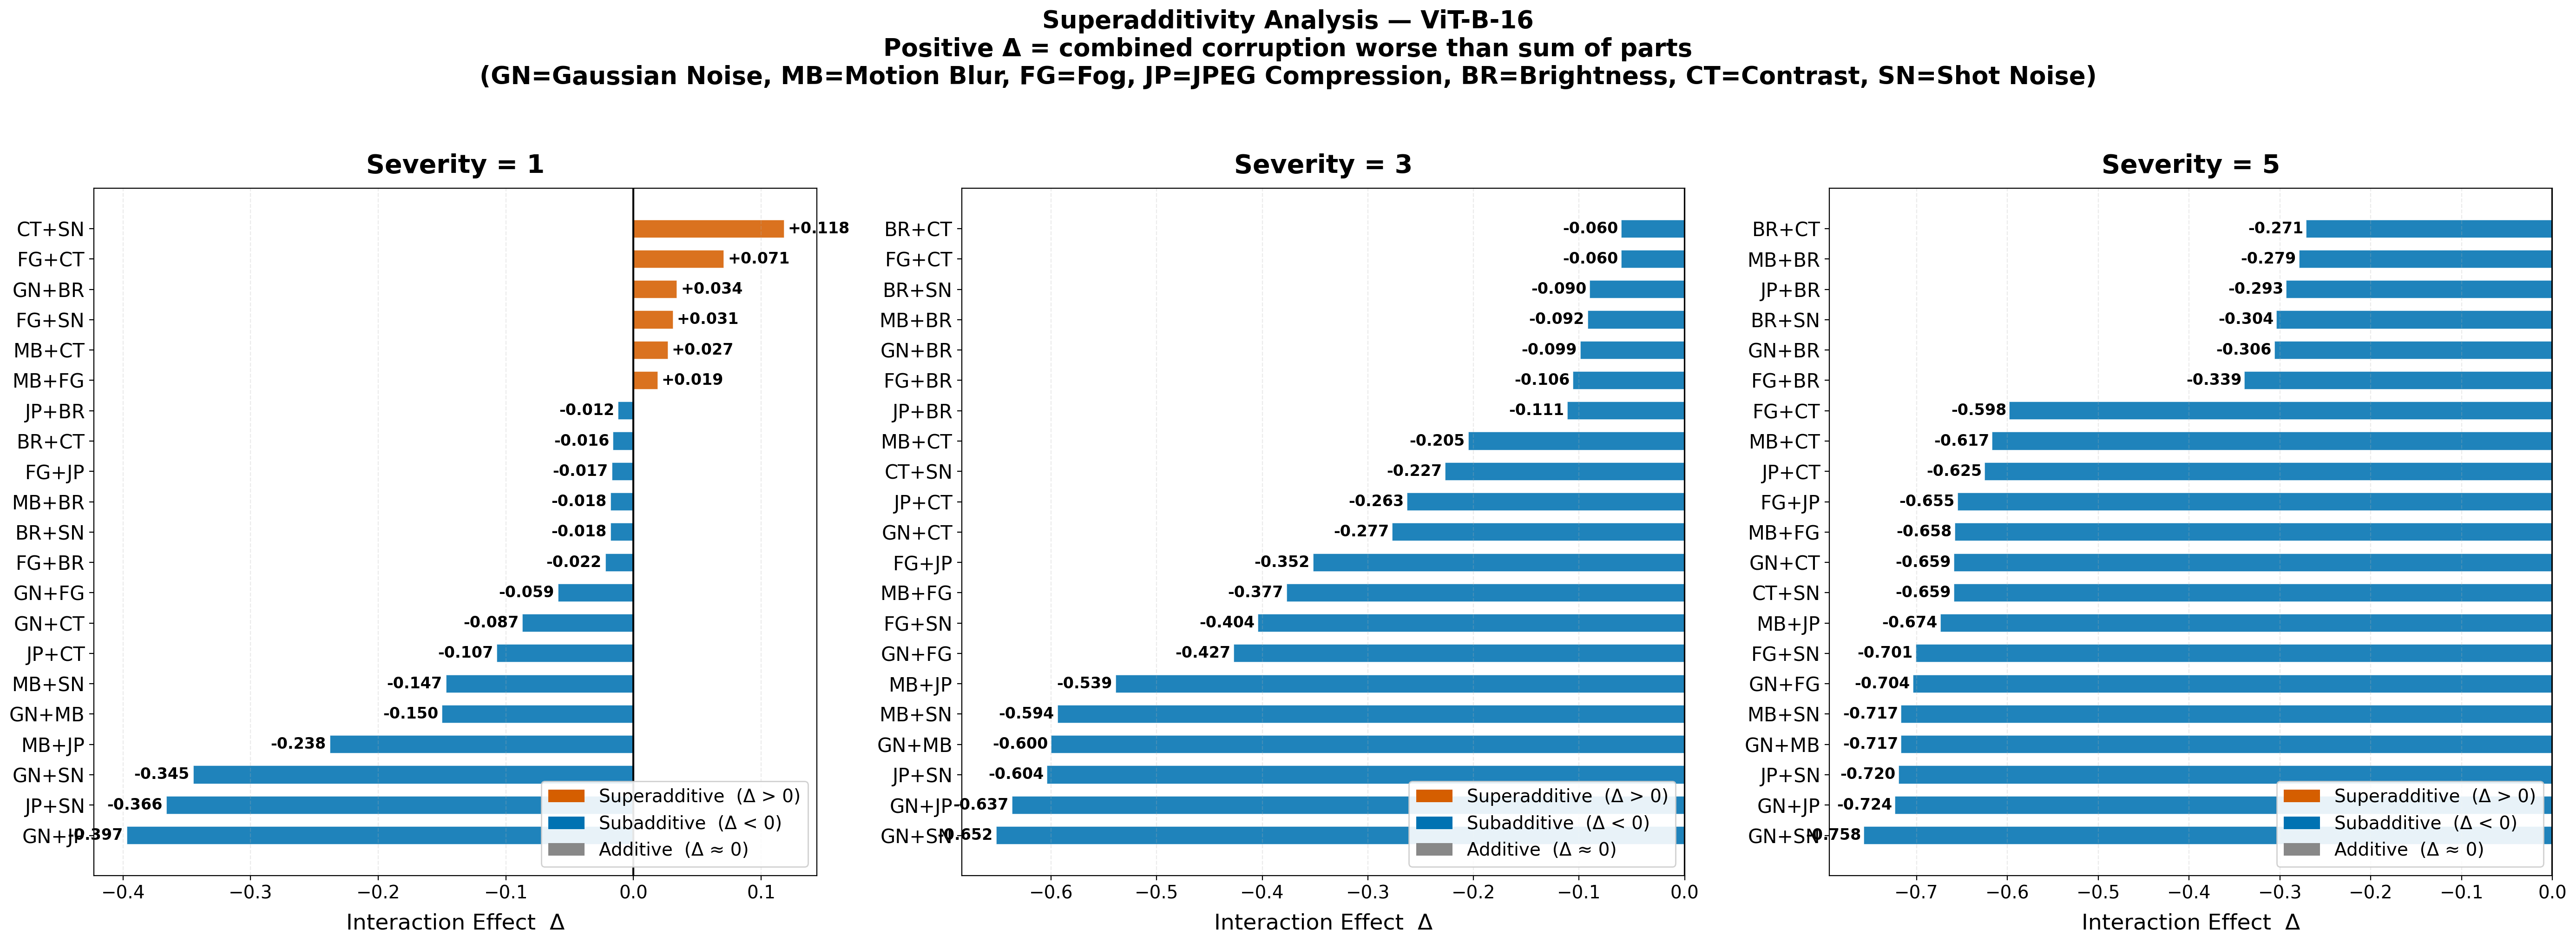
\includegraphics[width=\textwidth]{superadditivity_ViT-B-16.png}
    \caption{ViT-B/16}
  \end{subfigure}

  \vspace{6pt}

  \begin{subfigure}{\textwidth}
    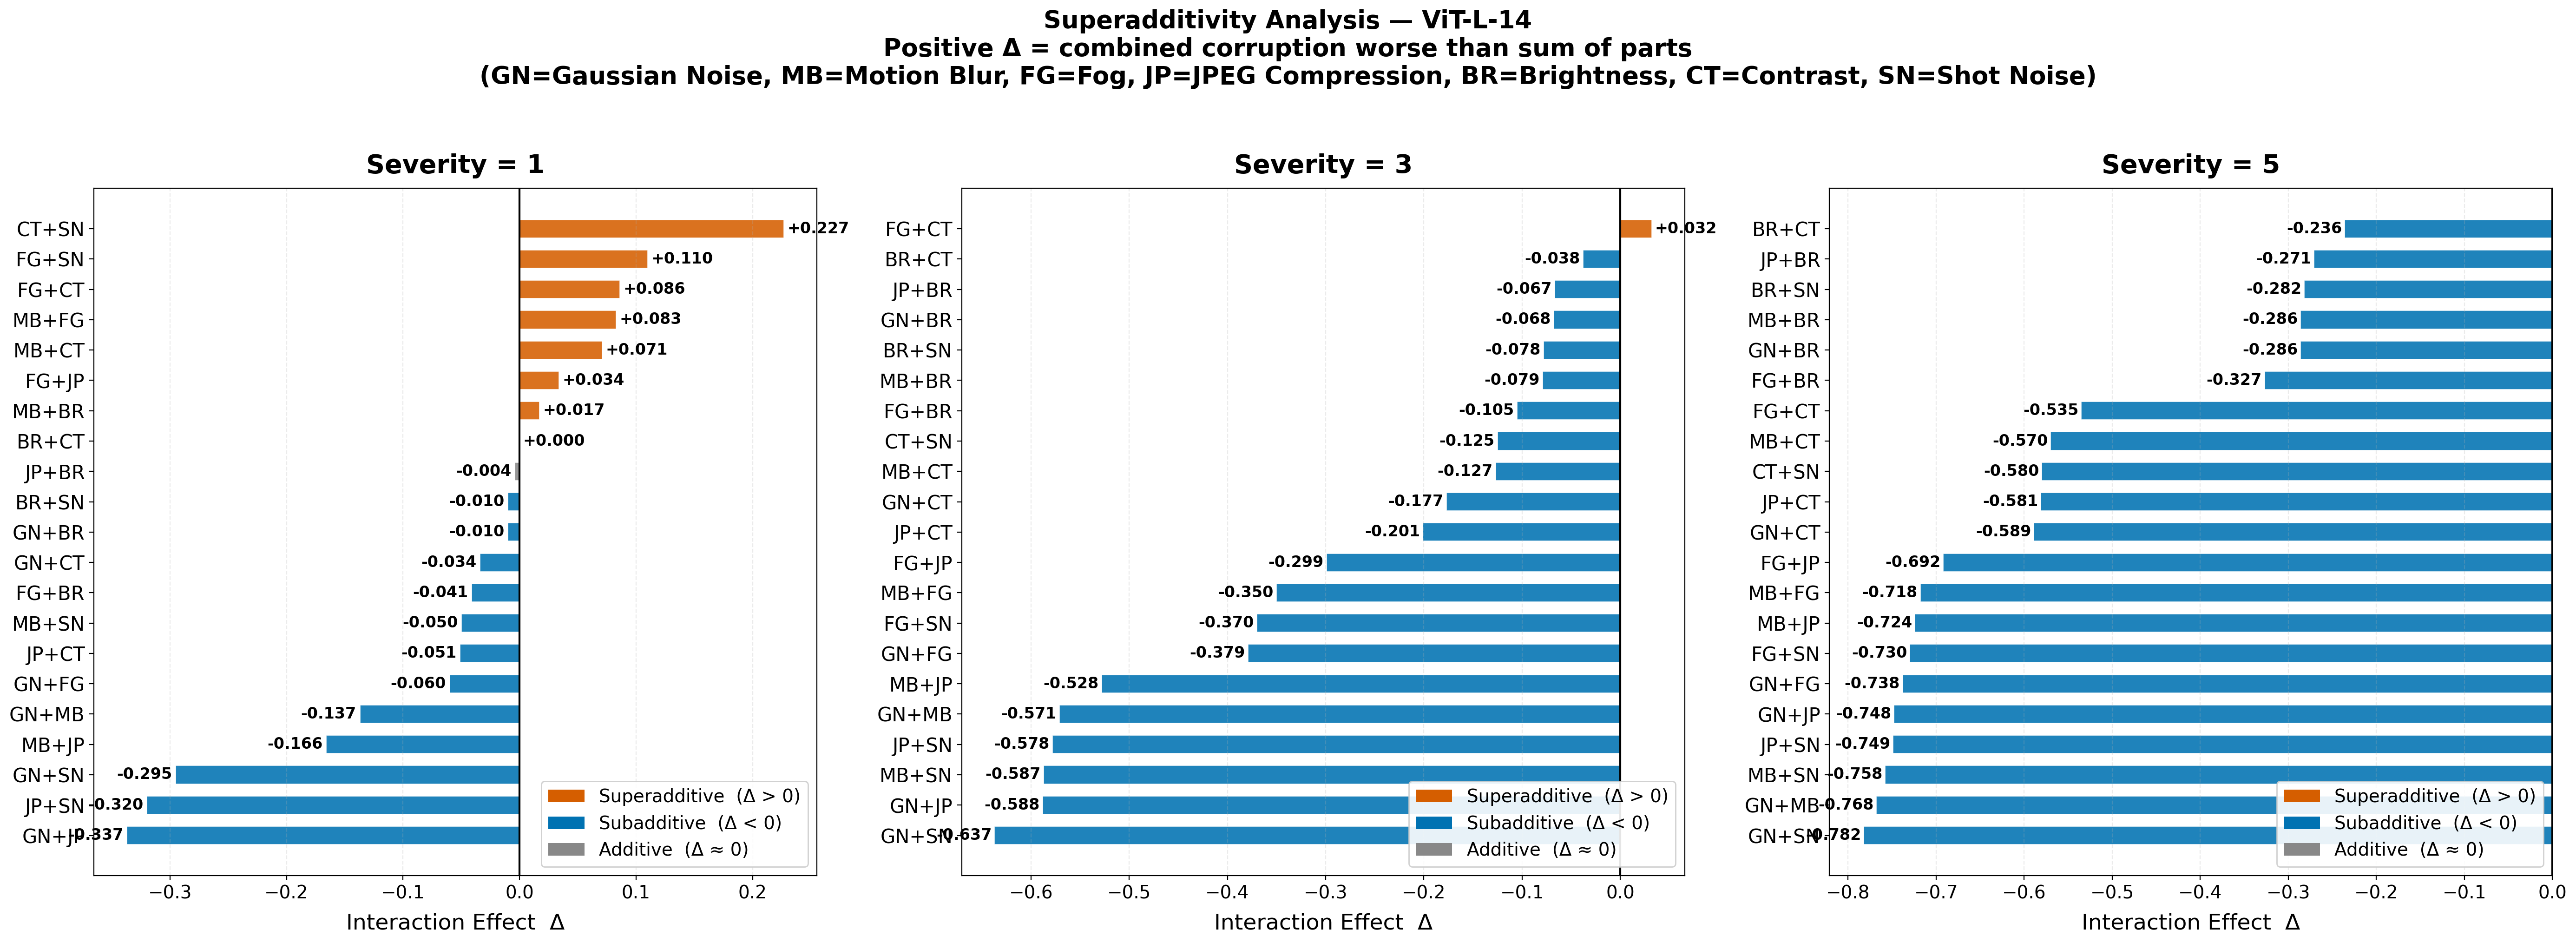
\includegraphics[width=\textwidth]{superadditivity_ViT-L-14.png}
    \caption{ViT-L/14}
  \end{subfigure}

  \caption{
    Interaction effect $\cI$ (\cref{eq:interaction})
    for all 21~corruption pairs across severity levels.
    \textcolor{supercolor}{\textbf{Red bars}}:
    superadditive ($\cI > 0$);
    \textcolor{subcolor}{\textbf{blue bars}}:
    subadditive ($\cI < 0$).
    ViT-L/14 exhibits significantly stronger positive
    interactions than smaller models.
    \textbf{Abbreviations:}
    GN=Gaussian Noise, MB=Motion Blur, FG=Fog,
    JP=JPEG Compression, BR=Brightness,
    CT=Contrast, SN=Shot Noise.
  }
  \label{fig:superadditivity}
\end{figure*}

% ============================================================================
% 5. DISCUSSION & LIMITATIONS
% ============================================================================
\section{Discussion \& Limitations}
\label{sec:discussion}

\paragraph{Why contrast\,+\,shot\_noise dominates.}
We hypothesise that these corruptions attack
\emph{complementary} feature channels.
Reduced contrast removes global luminance structure;
shot noise destroys local texture statistics.
CLIP's patch tokenisation relies on both for semantic
alignment---losing both simultaneously causes
catastrophic failure.

\paragraph{Why scale amplifies superadditivity.}
ViT-L/14's higher clean accuracy implies richer,
more complex feature representations with more
``ways to fail'' under compound perturbations.
This is an instance of the accuracy--robustness
trade-off under compound perturbations.

\paragraph{Limitations.}
\begin{itemize}[leftmargin=*]
  \item \textbf{Dataset.} CIFAR-100 ($32{\times}32$~px)
        is used as an ImageNet proxy due to access
        constraints; low resolution may exaggerate
        corruption effects.
        Replication on full ImageNet is a priority.
  \item \textbf{Corruption scope.} We evaluate 7 of
        15+ corruptions in ImageNet-C; extending to
        all types would yield a more complete
        interaction map.
  \item \textbf{Pair order.} We evaluate one fixed
        order per pair in the main study; order
        sensitivity is analysed in \cref{sec:rq4}
        for top-5 pairs only.
  \item \textbf{Beyond pairs.} Triplet and
        higher-order combinations remain unstudied.
  \item \textbf{No XAI.} Grad-CAM or attention
        visualisations under combined corruptions
        would provide mechanistic insight; we leave
        this for future work.
\end{itemize}

% ============================================================================
% 6. CONCLUSION
% ============================================================================
\section{Conclusion}
\label{sec:conclusion}

We presented the first systematic study of pairwise
corruption interactions for CLIP-family visual encoders.
Our interaction effect metric $\cI$ quantifies whether
combined corruptions are worse than the sum of their
parts.
Superadditivity is a genuine, reproducible phenomenon
at low severity, with \textbf{contrast\,+\,shot\_noise}
emerging as the most dangerous pair across all three
architectures.
Model scale \emph{does not} mitigate combined corruption
effects---larger models exhibit stronger superadditivity
due to higher clean accuracy.
Furthermore, corruption order critically determines
worst-case degradation, with gaps up to $0.21$ in
absolute accuracy for fixed-order protocols.

These results expose a systematic blind spot in current
VLM evaluation and motivate the adoption of
combined-corruption, multi-order benchmarking protocols.

% ============================================================================
% REFERENCES
% ============================================================================
% ВАЖНО: порядок именно такой:
%   1. \bibliographystyle
%   2. \bibliography
% И компилировать: pdflatex -> bibtex -> pdflatex -> pdflatex
\clearpage          % ← выталкивает ВСЕ отложенные float'ы на страницу
\bibliographystyle{IEEEtran}
\bibliography{references}

% ============================================================================
% APPENDIX
% ============================================================================
\appendix
\section{Additional Heatmaps}
\label{app:heatmaps}

\cref{fig:heatmaps_s3,fig:heatmaps_s5} show accuracy
drop heatmaps at severity levels $s=3$ and $s=5$.
At $s=3$, the noise-family corruptions have already
driven accuracy near zero; at $s=5$, virtually all
pairs exhibit subadditive behaviour due to floor
effects.

\begin{figure*}[h]
  \centering
  \begin{subfigure}[b]{0.32\textwidth}
    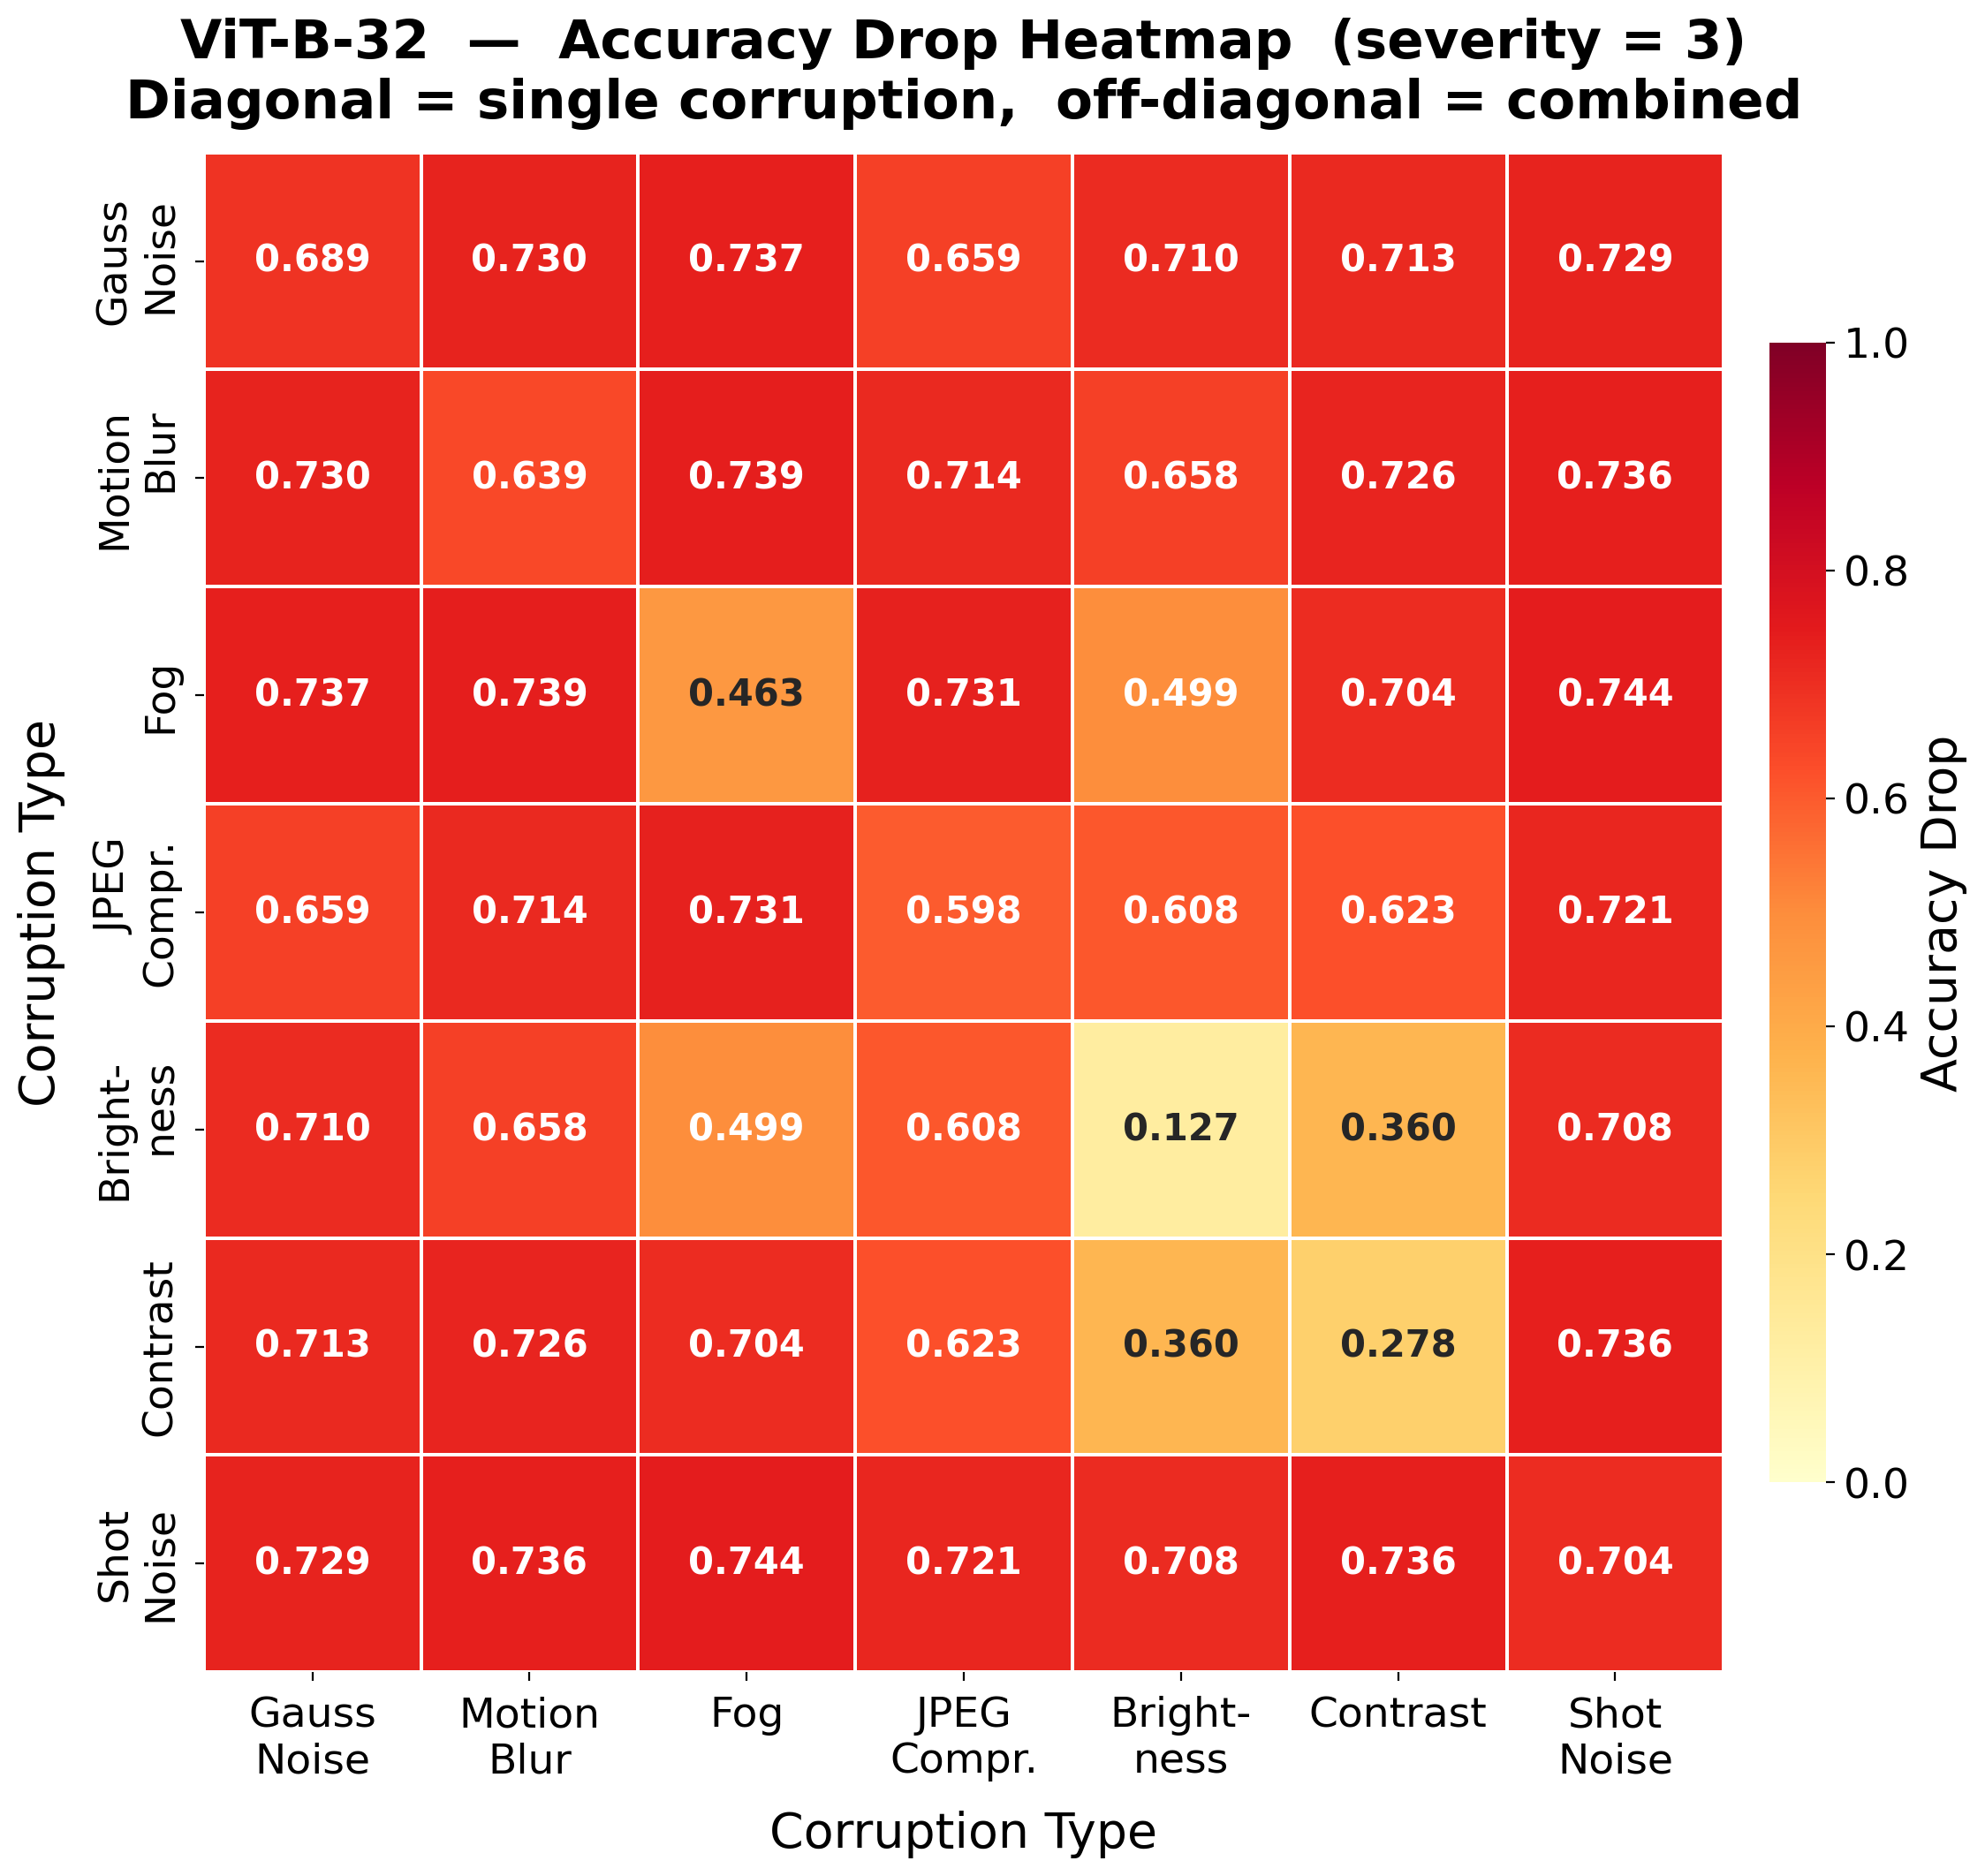
\includegraphics[width=\textwidth]{heatmap_ViT-B-32_s3.png}
    \caption{ViT-B/32, $s=3$}
  \end{subfigure}
  \hfill
  \begin{subfigure}[b]{0.32\textwidth}
    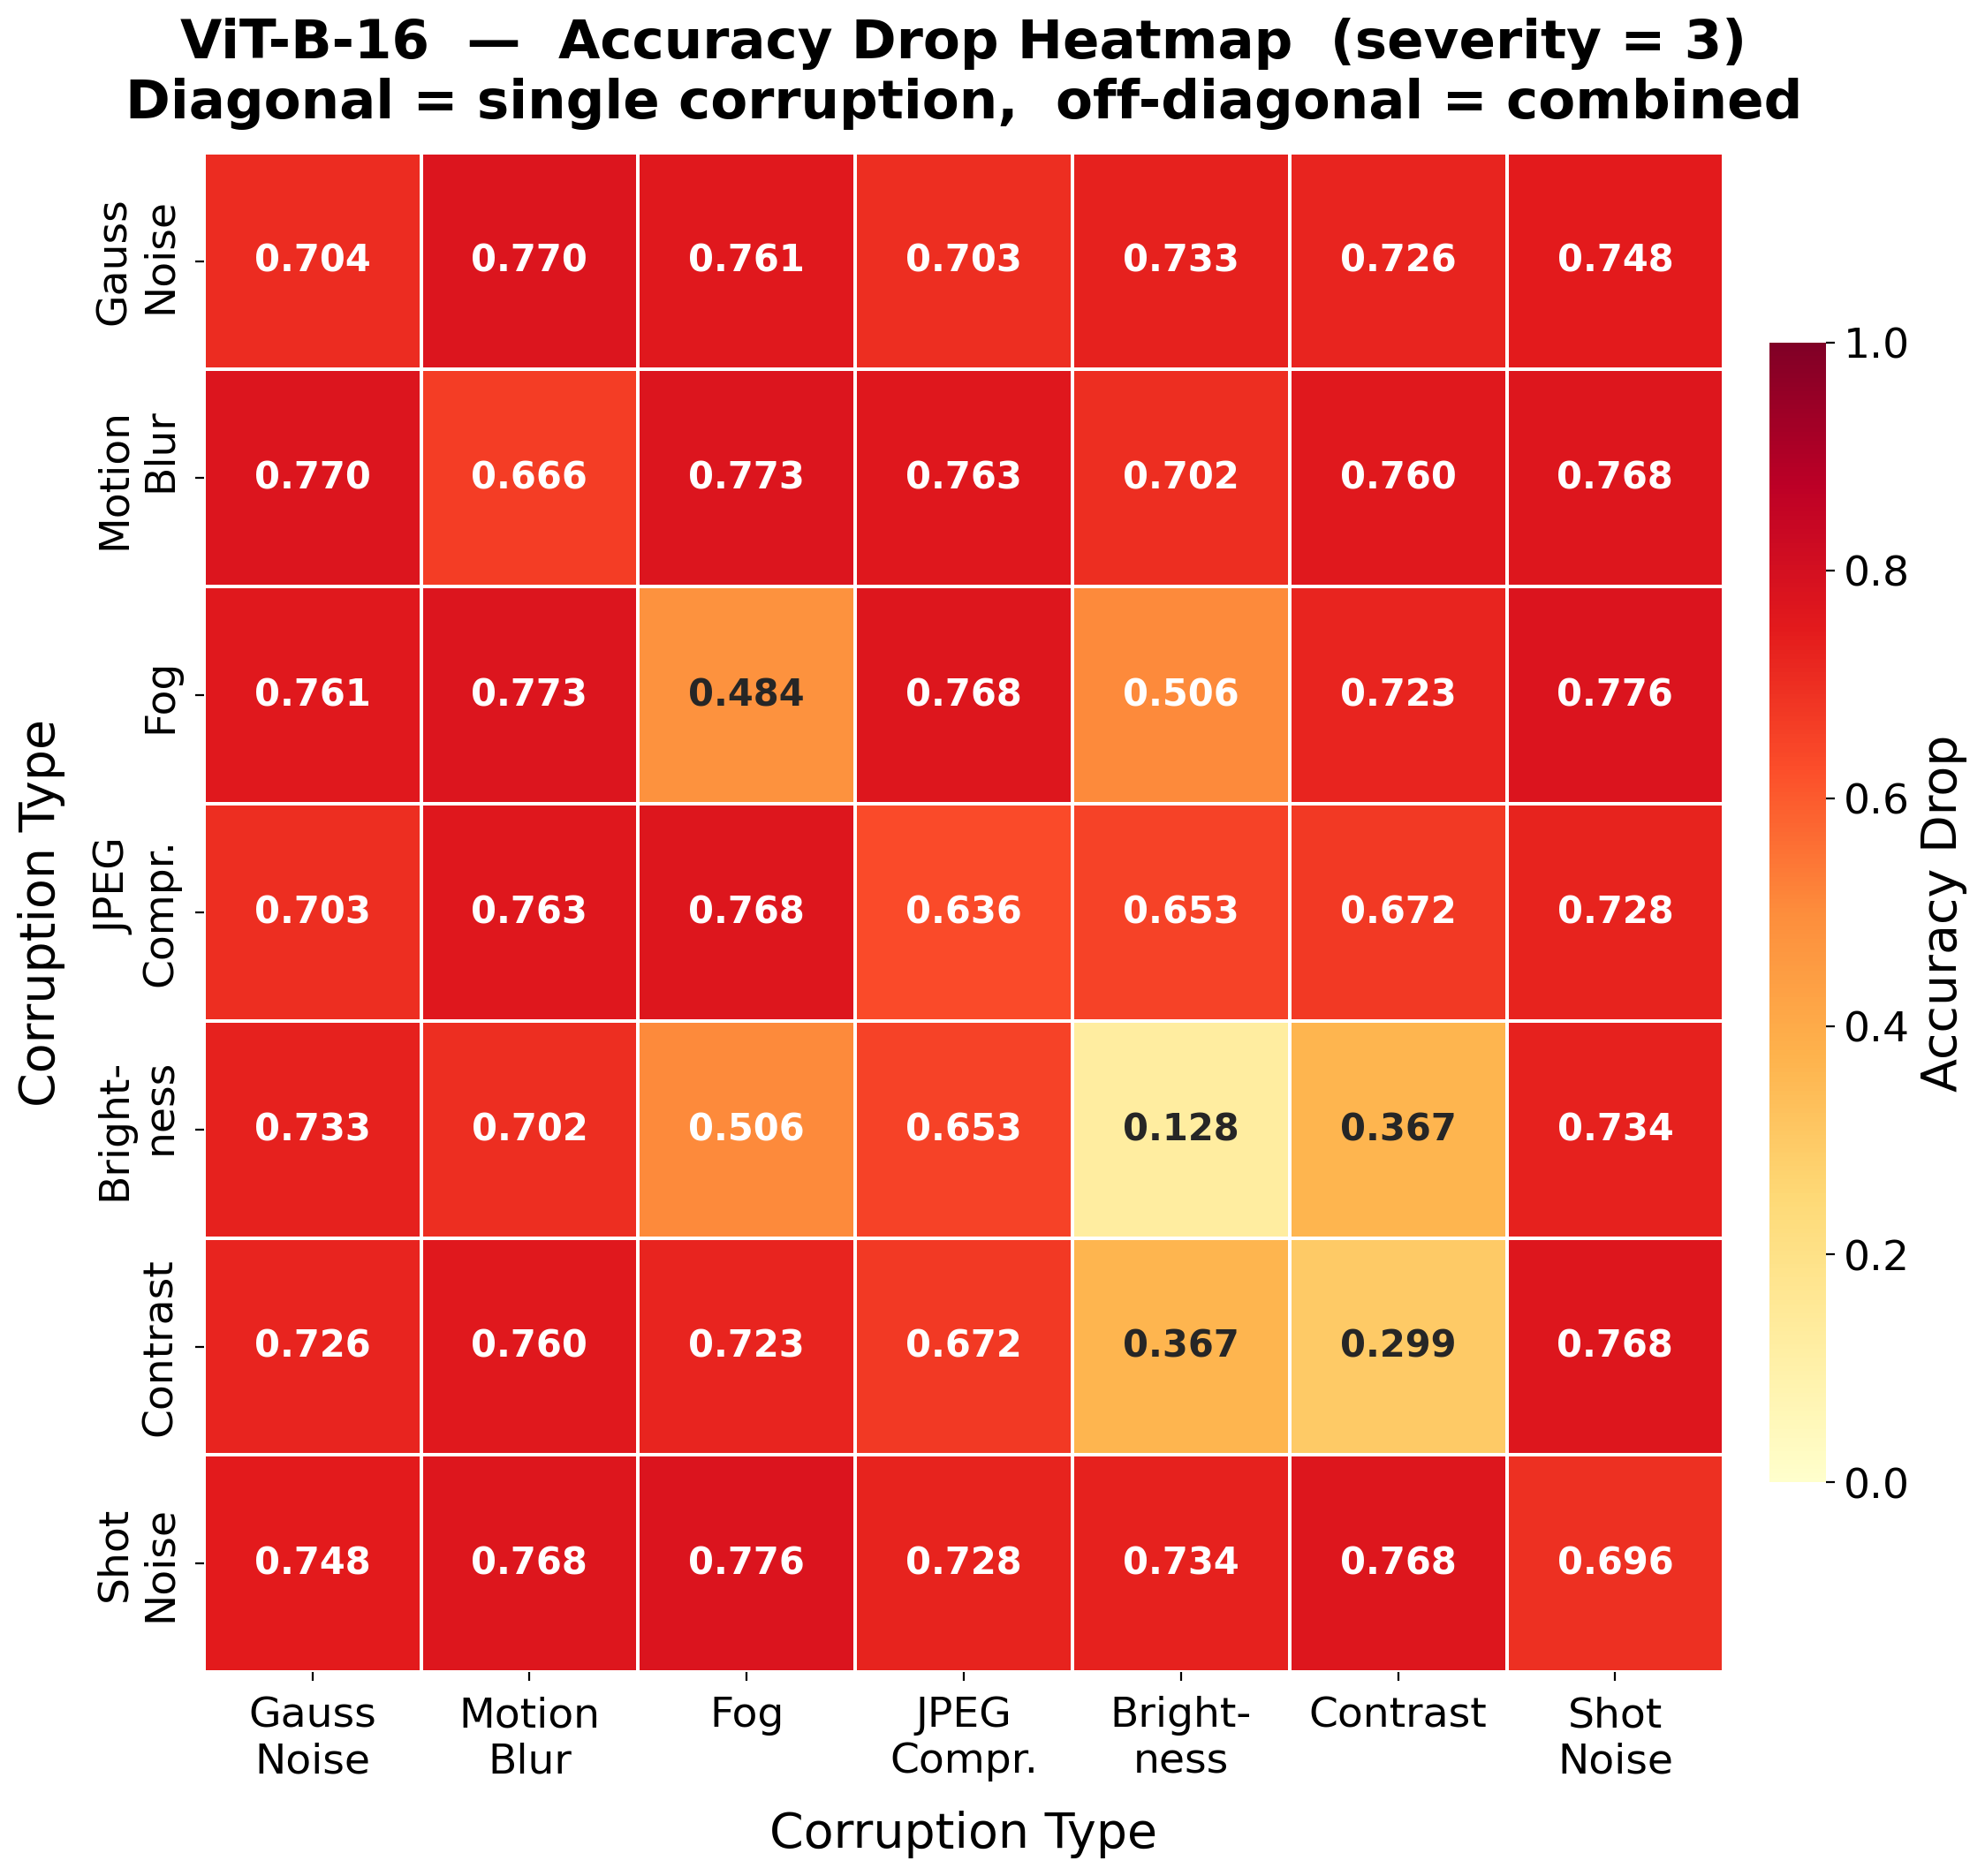
\includegraphics[width=\textwidth]{heatmap_ViT-B-16_s3.png}
    \caption{ViT-B/16, $s=3$}
  \end{subfigure}
  \hfill
  \begin{subfigure}[b]{0.32\textwidth}
    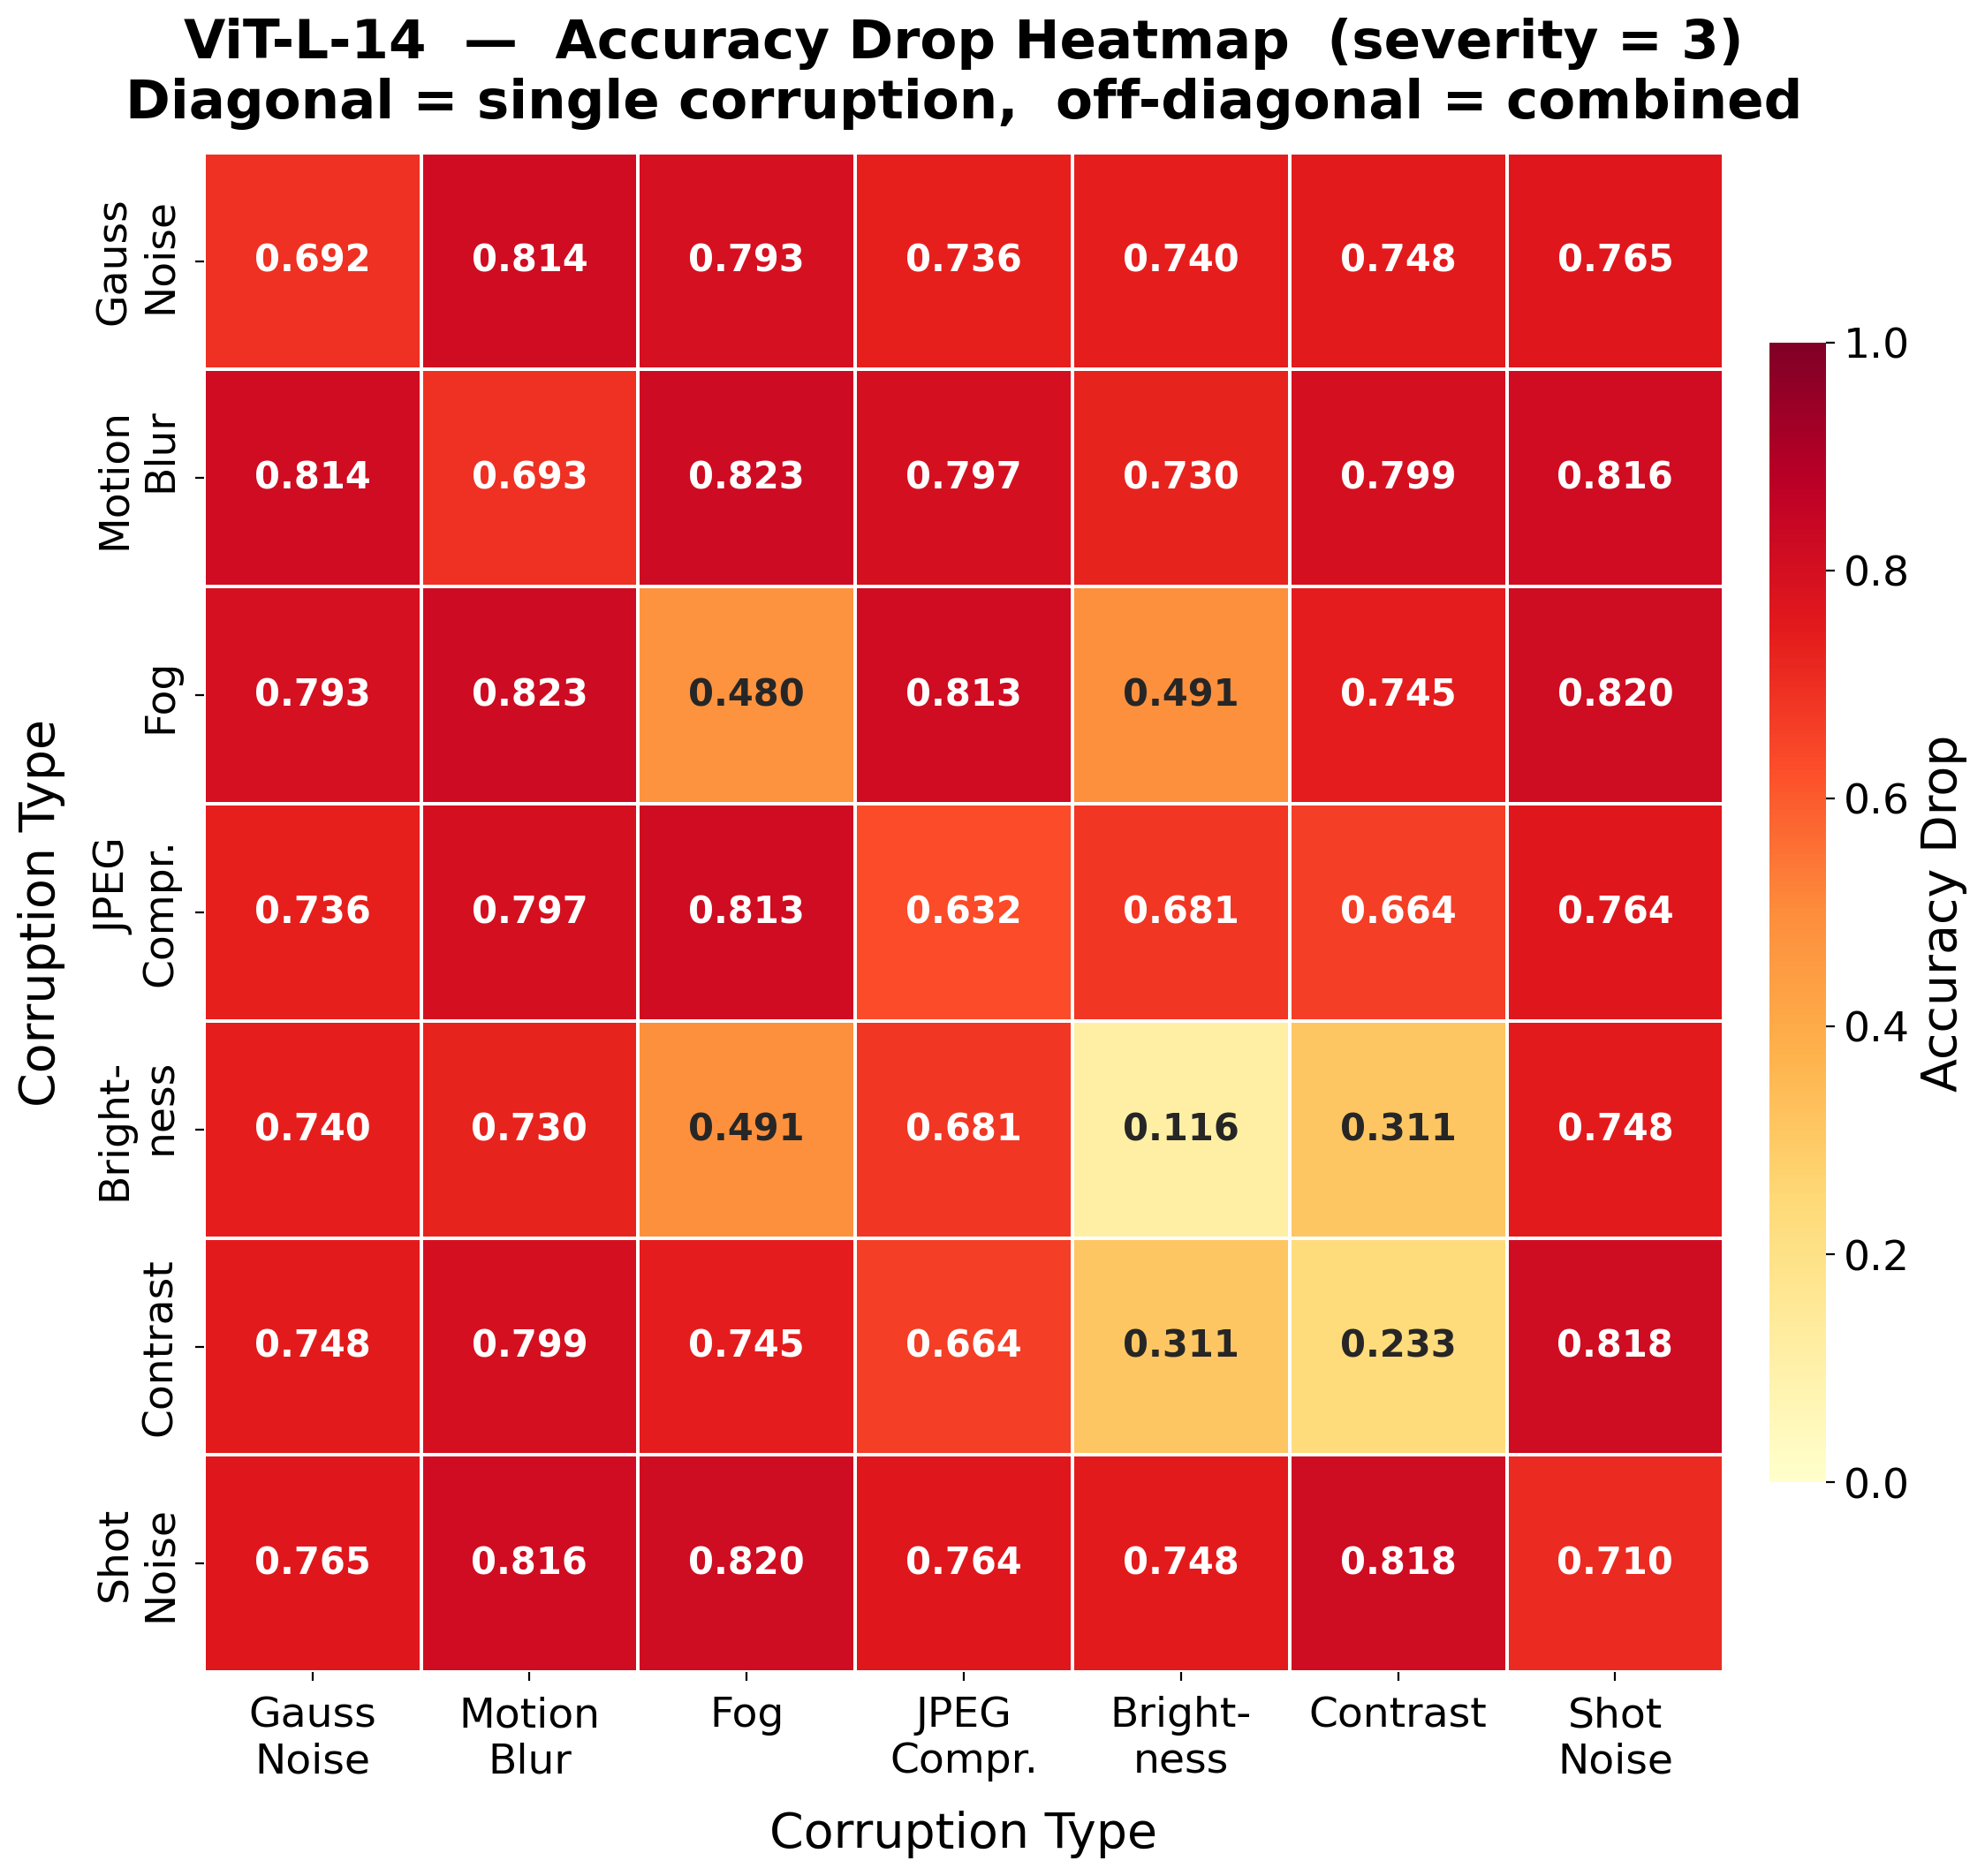
\includegraphics[width=\textwidth]{heatmap_ViT-L-14_s3.png}
    \caption{ViT-L/14, $s=3$}
  \end{subfigure}
  \caption{Accuracy drop heatmaps at severity $s=3$.}
  \label{fig:heatmaps_s3}
\end{figure*}

\begin{figure*}[h]
  \centering
  \begin{subfigure}[b]{0.32\textwidth}
    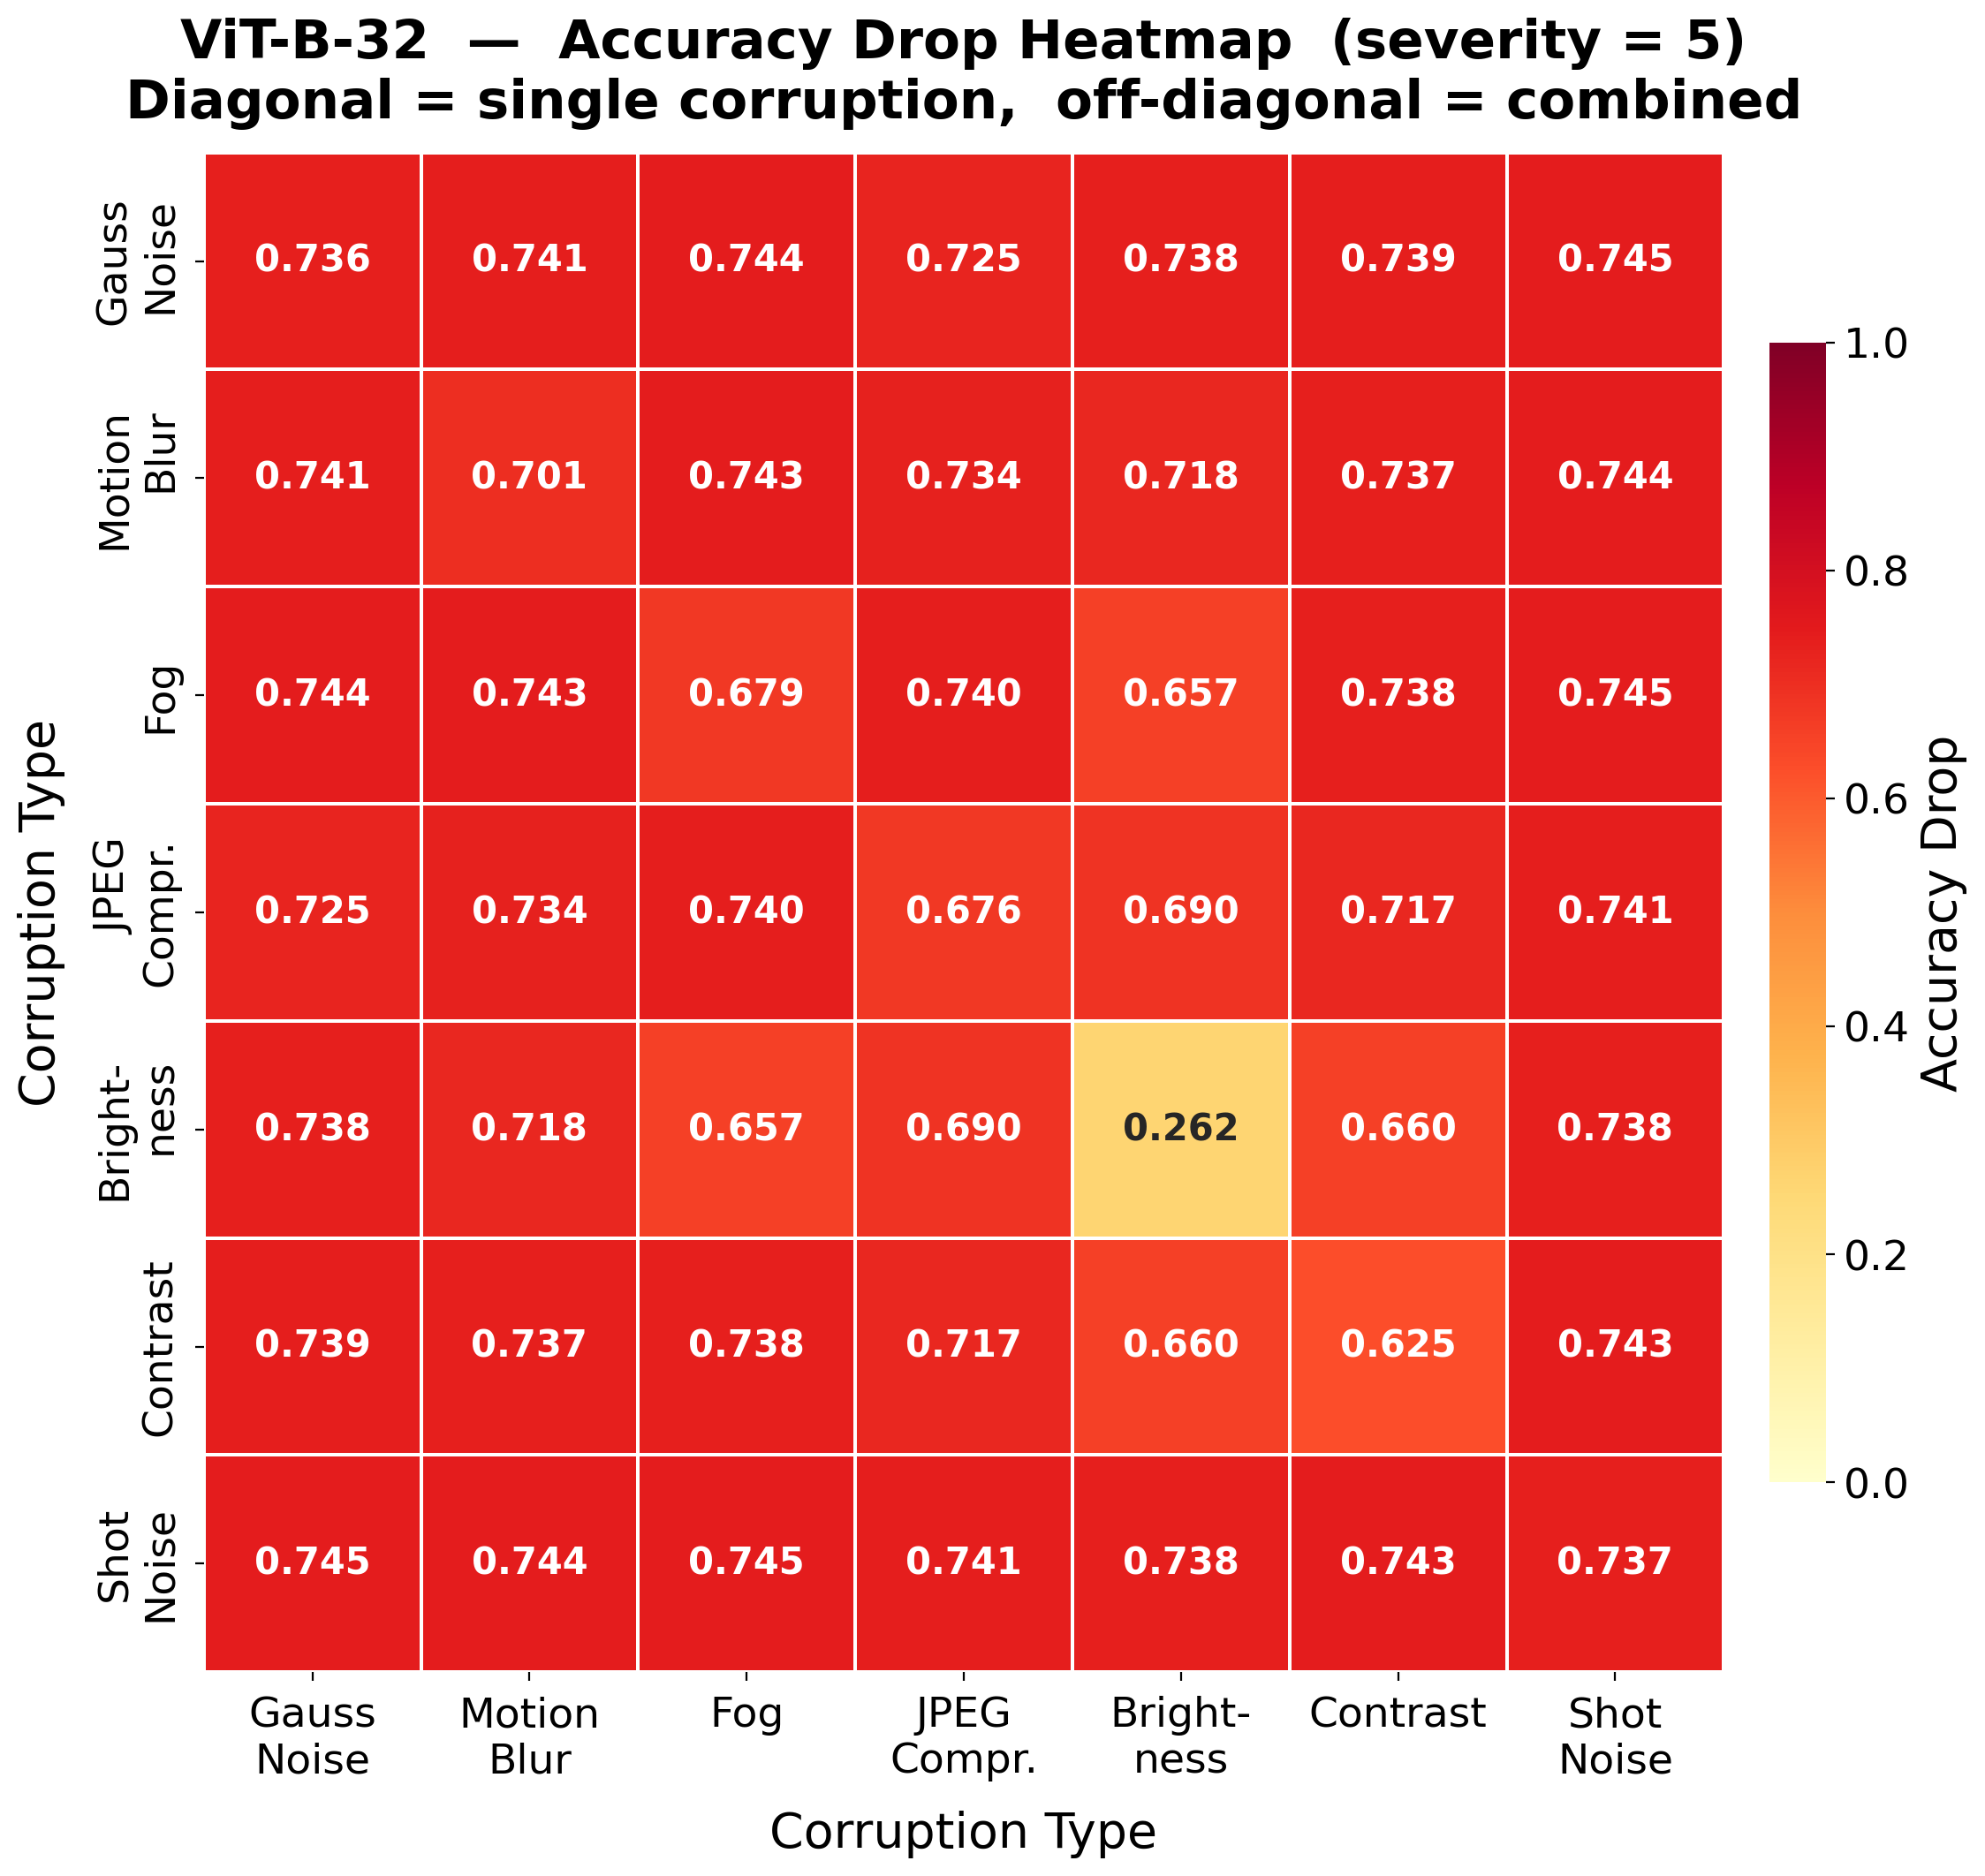
\includegraphics[width=\textwidth]{heatmap_ViT-B-32_s5.png}
    \caption{ViT-B/32, $s=5$}
  \end{subfigure}
  \hfill
  \begin{subfigure}[b]{0.32\textwidth}
    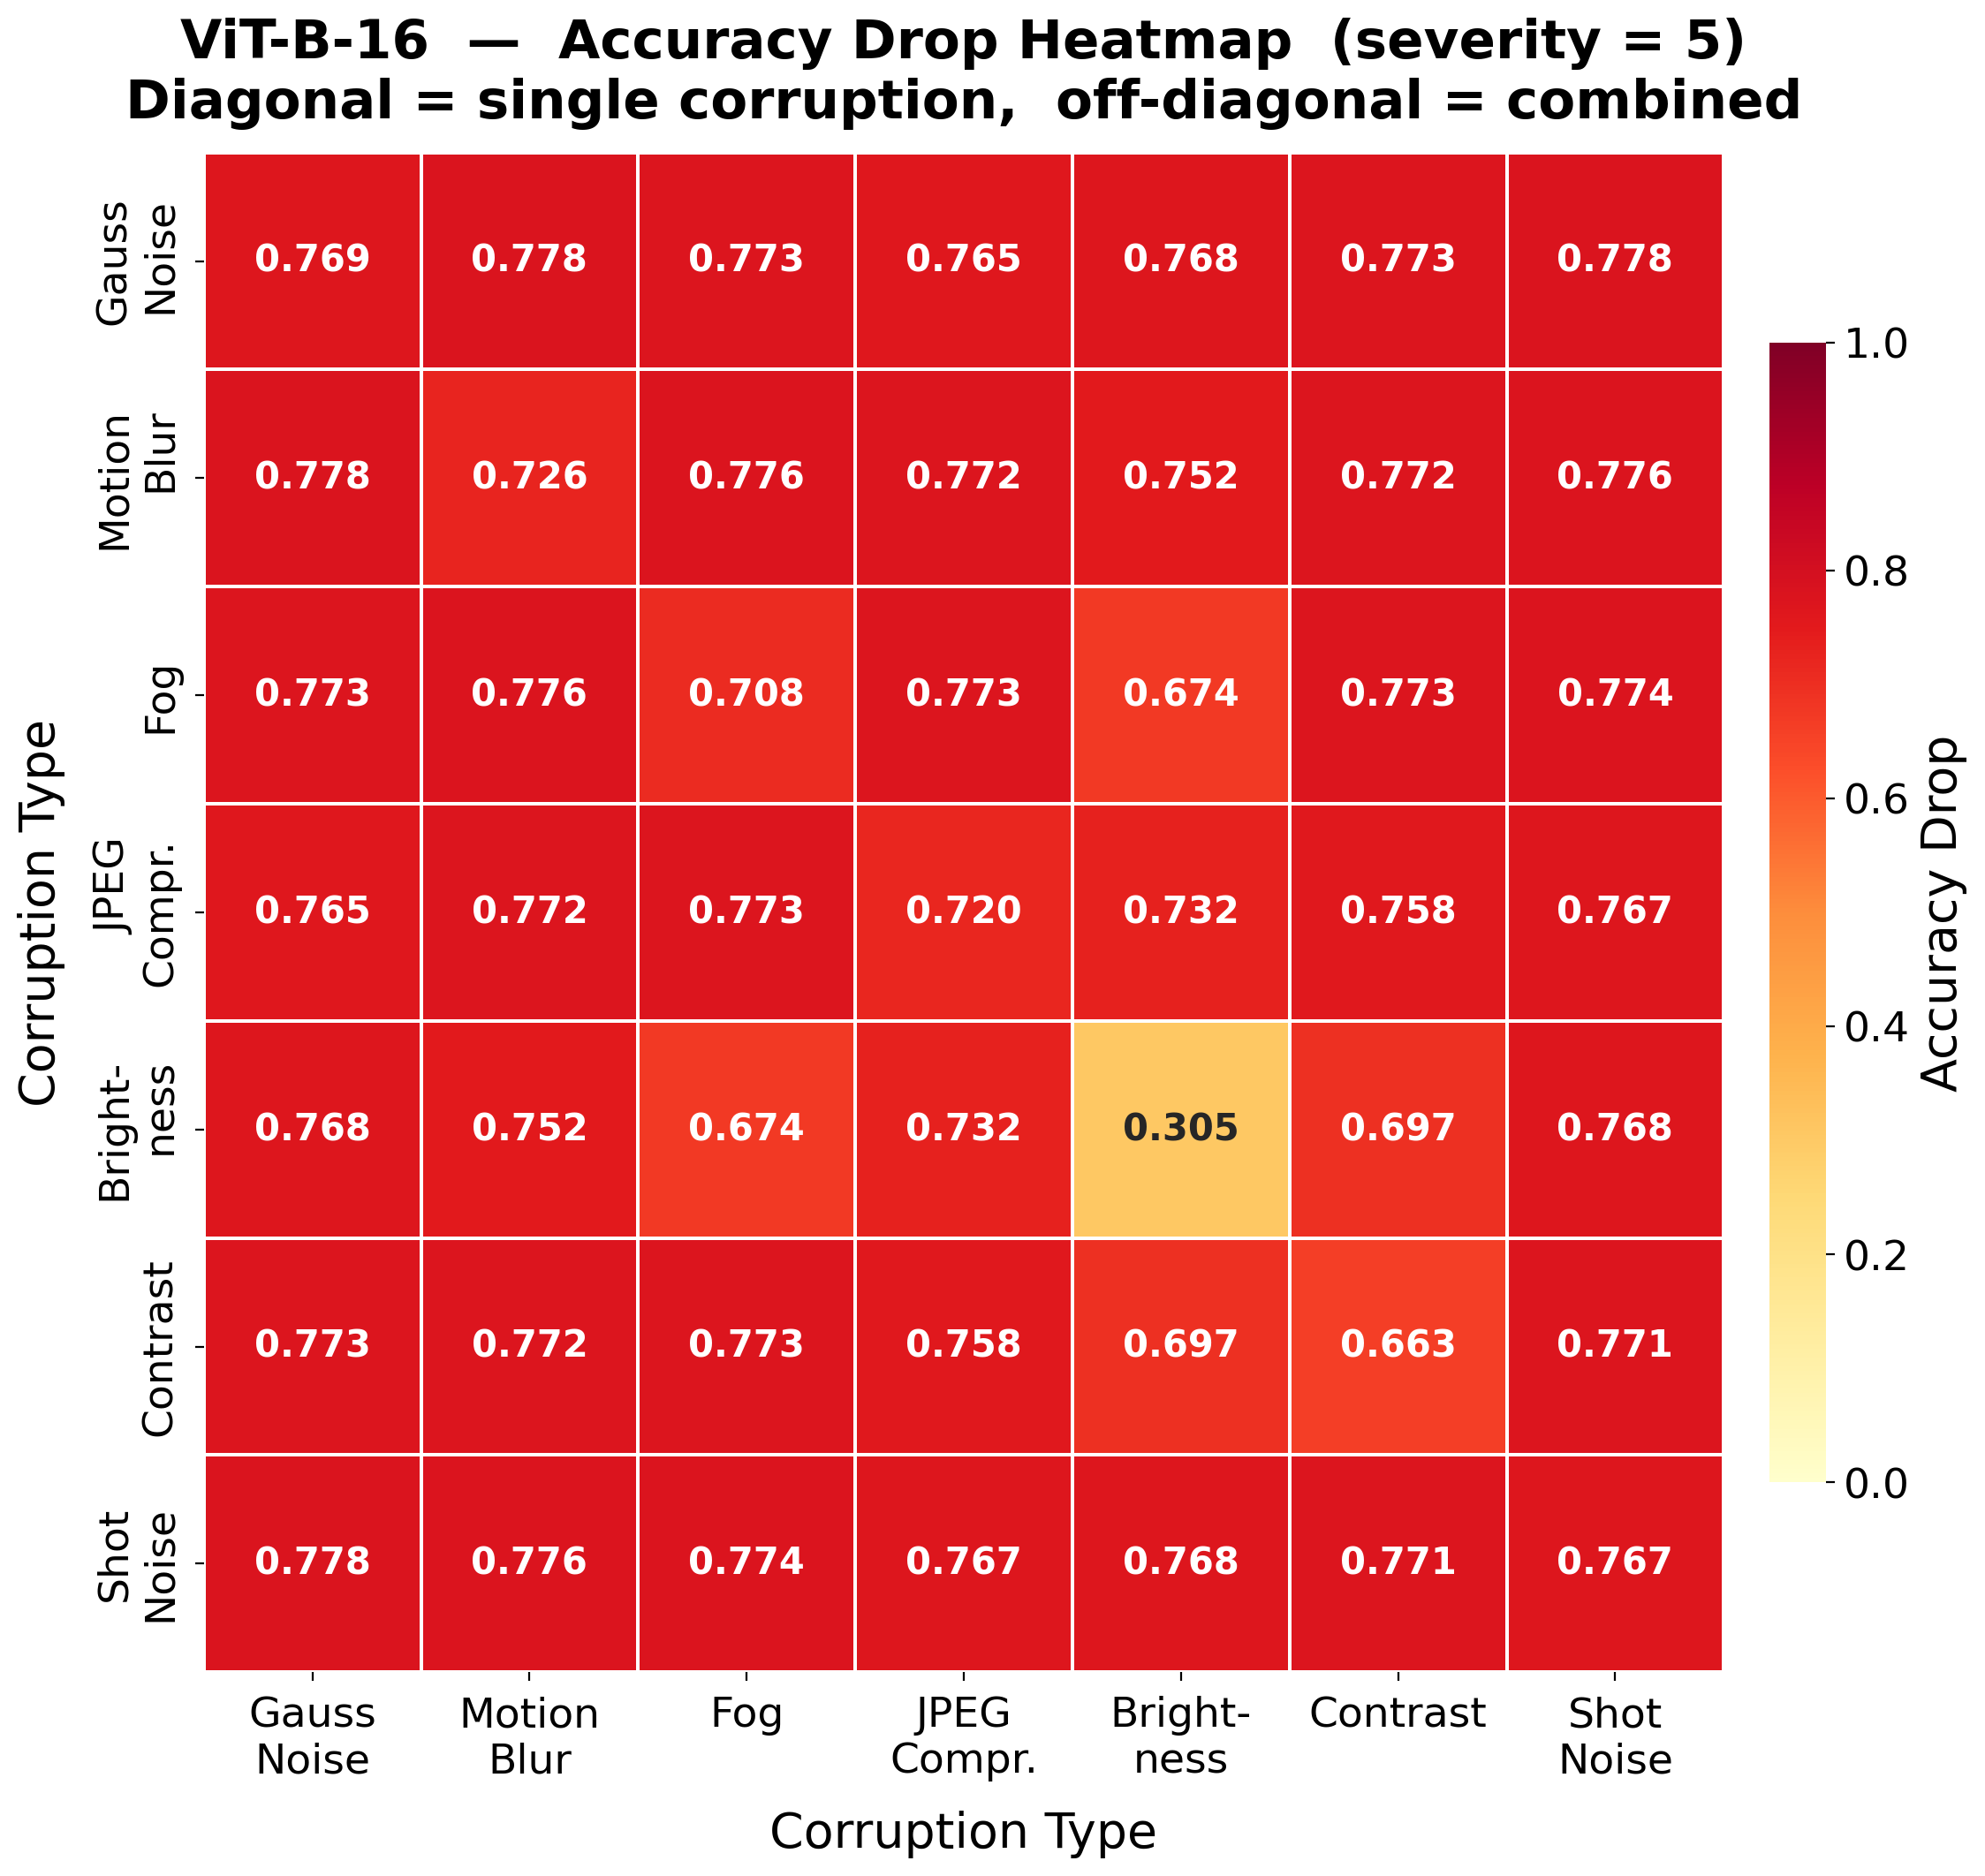
\includegraphics[width=\textwidth]{heatmap_ViT-B-16_s5.png}
    \caption{ViT-B/16, $s=5$}
  \end{subfigure}
  \hfill
  \begin{subfigure}[b]{0.32\textwidth}
    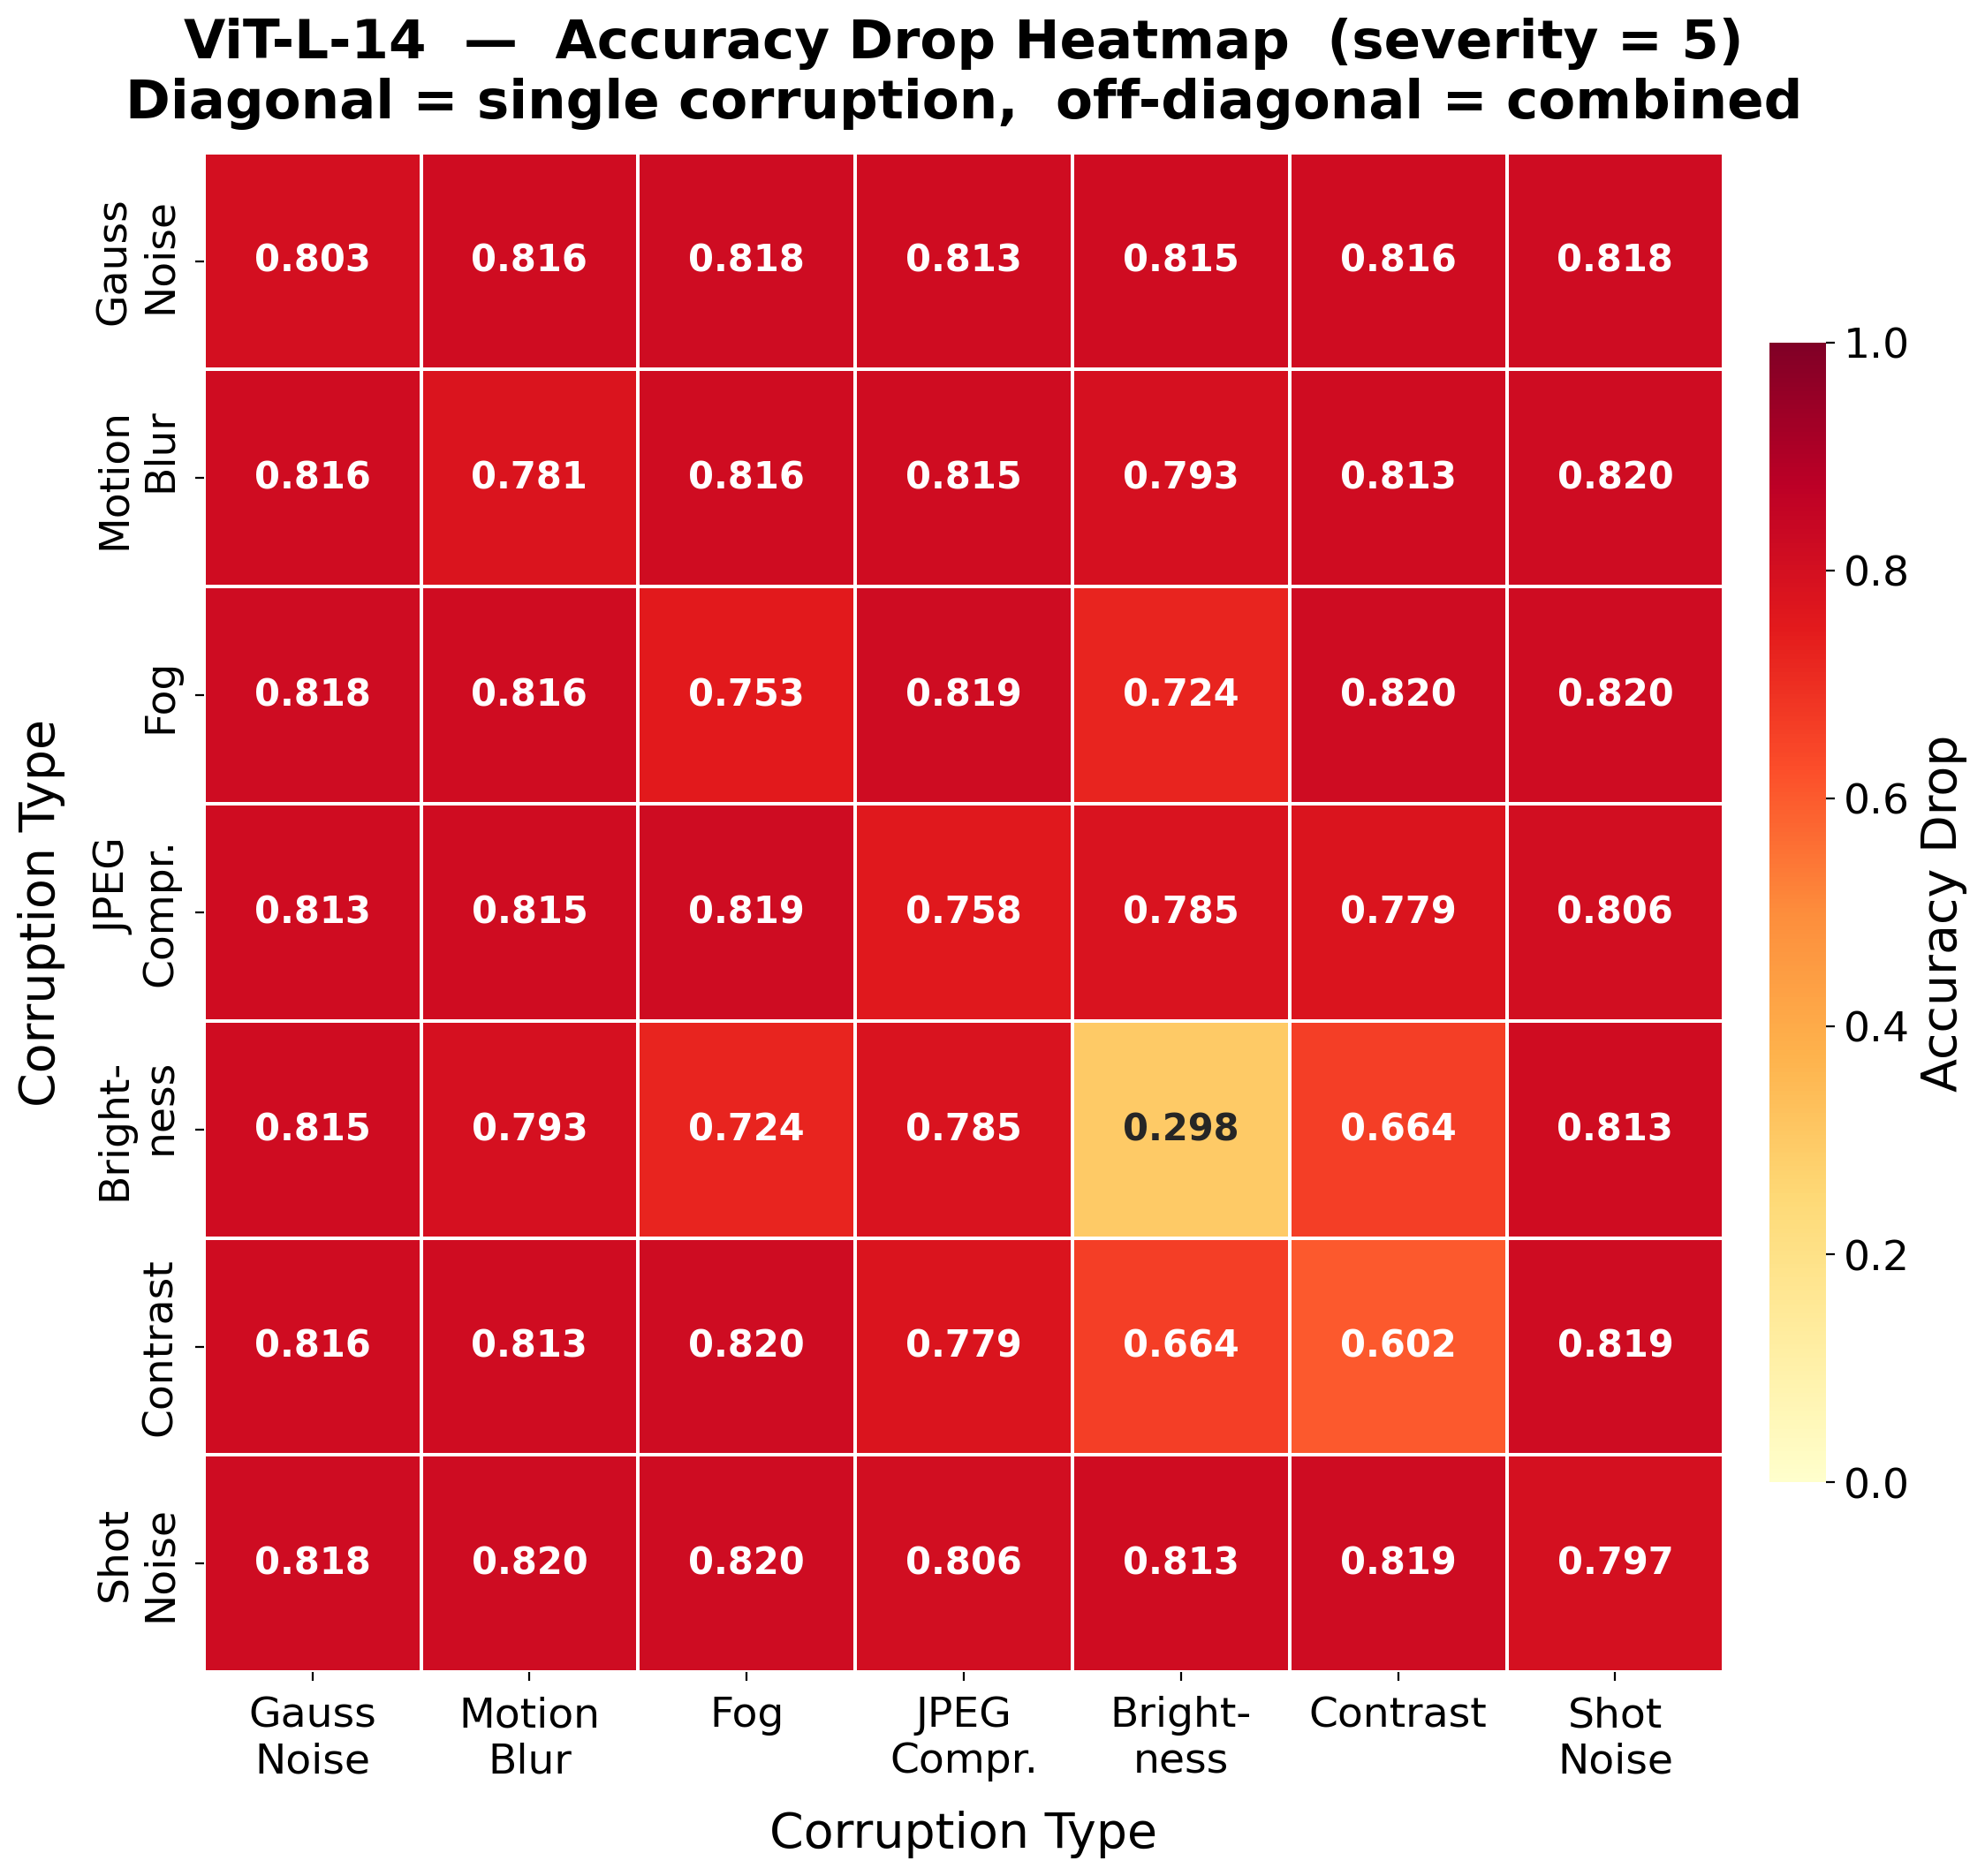
\includegraphics[width=\textwidth]{heatmap_ViT-L-14_s5.png}
    \caption{ViT-L/14, $s=5$}
  \end{subfigure}
  \caption{Accuracy drop heatmaps at severity $s=5$.}
  \label{fig:heatmaps_s5}
\end{figure*}

\end{document}